\documentclass[a4paper]{article}
\usepackage[utf8]{inputenc}
\usepackage{todonotes}
\usepackage[russian]{babel}
\usepackage{graphicx}
\usepackage{float}
\usepackage{wrapfig}
\usepackage{tikz}
\usepackage{amsmath, amssymb}
\usepackage{hyperref}
\usepackage{listings}
\usepackage{caption}
\usepackage{geometry}
\usepackage{fancyhdr}
\usepackage{nicefrac}
\usepackage{xcolor}

\geometry{left=2cm,right=2cm,top=2cm,bottom=2cm}
\definecolor{urlcolor}{rgb}{0,0,1}
\definecolor{linkcolor}{rgb}{0,0,0.8}
\hypersetup{pdfborder=0 0 0}
\hypersetup{pdfstartview=FitH, linkcolor=linkcolor, urlcolor=urlcolor, colorlinks=true}

\definecolor{strings}{rgb}{0,0.6,0}
\definecolor{comments}{rgb}{0,0.3,0}
\definecolor{numbers}{rgb}{0.5,0.5,0.5}
\definecolor{keywords}{rgb}{0.09,0.61,0.95}
\definecolor{background}{rgb}{0.97,0.97,0.97}

\lstdefinestyle{codestyle}{
    backgroundcolor=\color{background},
    commentstyle=\color{comments},
    keywordstyle=\color{keywords},
    stringstyle=\color{strings},
    numberstyle=\tiny\color{numbers},
    basicstyle=\ttfamily\footnotesize,
    breakatwhitespace=false,
    breaklines=true,
    captionpos=b,
    inputencoding=utf8,
    keepspaces=true,
    numbers=left,
    numbersep=5pt,
    showspaces=false,
    showstringspaces=false,
    showtabs=false,
    tabsize=2,
    extendedchars=true,
    literate=
      {а}{{\cyra}}1 {б}{{\cyrb}}1 {в}{{\cyrv}}1 {г}{{\cyrg}}1
      {д}{{\cyrd}}1 {е}{{\cyre}}1 {ж}{{\cyrzh}}1 {з}{{\cyrz}}1
      {и}{{\cyri}}1 {й}{{\cyrishrt}}1 {к}{{\cyrk}}1 {л}{{\cyrl}}1
      {м}{{\cyrm}}1 {н}{{\cyrn}}1 {о}{{\cyro}}1 {п}{{\cyrp}}1
      {р}{{\cyrr}}1 {с}{{\cyrs}}1 {т}{{\cyrt}}1 {у}{{\cyru}}1
      {ф}{{\cyrf}}1 {х}{{\cyrh}}1 {ц}{{\cyrc}}1 {ч}{{\cyrch}}1
      {ш}{{\cyrsh}}1 {щ}{{\cyrshch}}1 {ъ}{{\cyrhrdsn}}1 {ы}{{\cyrery}}1
      {ь}{{\cyrsftsn}}1 {э}{{\cyrerev}}1 {ю}{{\cyryu}}1 {я}{{\cyrya}}1
      {А}{{\CYRA}}1 {Б}{{\CYRB}}1 {В}{{\CYRV}}1 {Г}{{\CYRG}}1
      {Д}{{\CYR96}}1 {Е}{{\CYRE}}1 {Ж}{{\CYRZH}}1 {З}{{\CYRZ}}1
      {И}{{\CYRI}}1 {Й}{{\CYRISHRT}}1 {К}{{\CYRK}}1 {Л}{{\CYRL}}1
      {М}{{\CYRM}}1 {Н}{{\CYRN}}1 {О}{{\CYRO}}1 {П}{{\CYRP}}1
      {Р}{{\CYRR}}1 {С}{{\CYRS}}1 {Т}{{\CYRT}}1 {У}{{\CYRU}}1
      {Ф}{{\CYRF}}1 {Х}{{\CYRH}}1 {Ц}{{\CYRC}}1 {Ч}{{\CYRCH}}1
      {Ш}{{\CYRSH}}1 {Щ}{{\CYRSHCH}}1 {Ъ}{{\CYRHRDSN}}1 {Ы}{{\CYRERY}}1
      {Ь}{{\CYRSFTSN}}1 {Э}{{\CYREREV}}1 {Ю}{{\CYRYU}}1 {Я}{{\CYRYA}}1
}

\lstset{style=codestyle}

\newcommand{\addsection}[1]{
    \phantomsection
    \addcontentsline{toc}{section}{#1}
    \section*{#1}
}
\newcommand{\addsubsection}[1]{
    \phantomsection
    \addcontentsline{toc}{subsection}{#1}
    \subsection*{#1}
}
\newcommand{\addsubsubsection}[1]{
    \phantomsection
    \addcontentsline{toc}{subsubsection}{#1}
    \subsubsection*{#1}
}

\begin{document}

\begin{titlepage}
    \centering
    {\large Федеральное государственное автономное образовательное учреждение\par}
    {\large высшего образования\par}
    {\bfseries САНКТ-ПЕТЕРБУРГСКИЙ НАЦИОНАЛЬНЫЙ ИССЛЕДОВАТЕЛЬСКИЙ УНИВЕРСИТЕТ ИТМО\par}
    {\bfseries Факультет систем управления и робототехники\par}
    \vfill
    {\Large \bfseries Лабораторная работа №5\par}
    {\Large \bfseries Связь непрерывного и дискретного\par}
    \vfill
    
    \begin{flushright}
        Студент: Сайфуллин Д.Р. \\
        Поток: ЧАСТ.МЕТ. R23 1.5 \\ 
        Преподаватели: Перегудин А.А.\\
        Догадин  Е.В.
    \end{flushright}
    \vfill
    Санкт-Петербург \\
    2025 г.
\end{titlepage}

\tableofcontents
\newpage

\addsection{Задание 1. Непрерывное и дискретное преобразование Фурье}
Для выполнения задания необходимо рассмотреть прямоугольную функцию:
\[
  \Pi(t) =
  \begin{cases}
    1, & |t| \leq \frac{1}{2}, \\
    0, & |t| > \frac{1}{2}.
  \end{cases}
\]
Фурье-преобразование функции $\Pi(t)$ определяется следующим интегралом:
\[
  \hat{\Pi}(\nu) = \int_{-\infty}^{+\infty} \Pi(t) e^{-2\pi i \nu t}\, dt.
\]
Так как $\Pi(t)$ отлична от нуля только в интервале $\left[-\frac{1}{2},\frac{1}{2}\right]$, интеграл можно записать в виде:
\[
  \hat{\Pi}(\nu)=\int_{-1/2}^{1/2} e^{-2\pi i \nu t}\, dt.
\]
Вычислим данный интеграл:
\[
  \hat{\Pi}(\nu)= \left. \frac{e^{-2\pi i \nu t}}{-2\pi i \nu} \right|_{t=-1/2}^{t=1/2}
  =\frac{1}{-2\pi i \nu}\left(e^{-2\pi i \nu \cdot \frac{1}{2}} - e^{2\pi i \nu \cdot \frac{1}{2}}\right).
\]
Заметим, что:
\[
  e^{-ix} - e^{ix} = -2i\sin x.
  \]
  Подставляем, где $x=\pi \nu$, и получаем:
  \[
\hat{\Pi}(\nu)= \frac{1}{-2\pi i \nu}\left(-2i\sin(\pi \nu)\right)
=\frac{2i\sin(\pi \nu)}{2\pi i \nu}
=\frac{\sin(\pi \nu)}{\pi \nu}.
\]
Таким образом, аналитический вид Фурье-образа функции $\Pi(t)$ имеет вид:
\[
  \boxed{\hat{\Pi}(\nu)=\frac{\sin(\pi \nu)}{\pi \nu}}.
\]
Эта функция является \emph{sinc}-функцией.
Построим график функции $\Pi(t)$ и её Фурье-образа $\hat{\Pi}(\nu)$:

\begin{figure}[H]
    \centering
    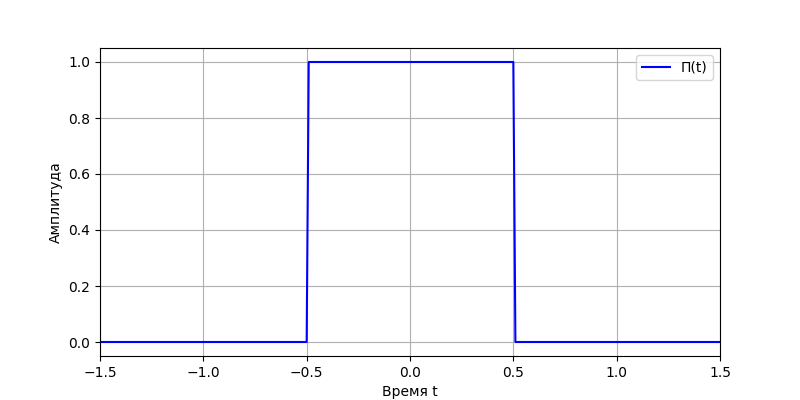
\includegraphics[width=0.8\textwidth]{src/task_1_0/time_f.png}
    \caption{График функции $\Pi(t)$.}
\end{figure}
\begin{figure}[H]
  \centering
  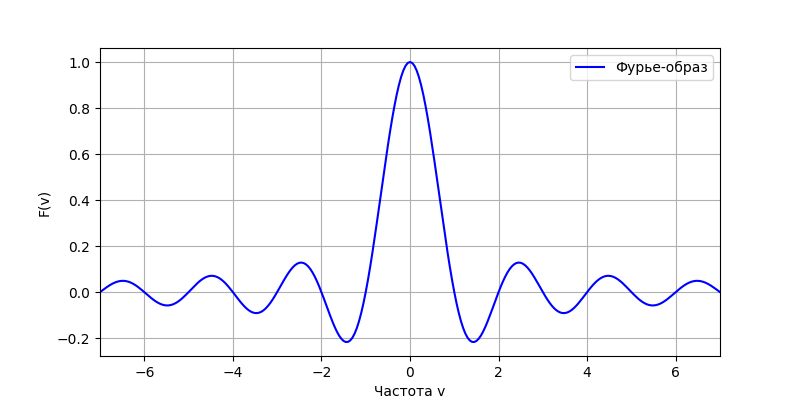
\includegraphics[width=0.8\textwidth]{src/task_1_0/freq_f.png}
  \caption{График Фурье-образа $\hat{\Pi}(\nu)$.}
\end{figure}

\addsubsection{Численное интегрирование}
В этом пункте мы будем использовать метод трапеций для численного интегрирования функции $\Pi(t)$ и её Фурье-образа $\hat{\Pi}(\nu)$. При вычислениях будем варьировать параметры для получения лучшего результата: сначала значения диапазона частот $V = \{5, 20\}$, затем шаг дискретизации во временной области $\Delta t = \{0.01, 0.0005\}$, интервал времени $T = \{5, 50\}$ и, наконец, шаг дискретизации в частотной области $\Delta \nu = \{0.02, 0.5\}$.

Начнем эксперентировать и посмотрим, как изменяются графики при различных значениях диапазона частот $V$. Для этого зададим диапазон частот $V=5$ и $V=20$ и посмотрим на результаты. Также посчитаем время, которое алгоритм затрачивает на преобразование и запишем его как $t$.

\begin{figure}[H]
  \centering
  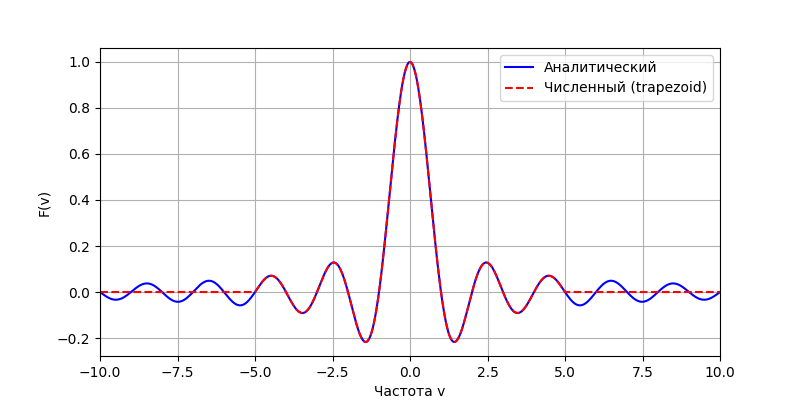
\includegraphics[width=\textwidth]{src/task_1_1/freq_5_0.01_5_0.02.png}
  \caption{Сравнительный график образов при $V=5$, $\Delta t=0.01$, $T=5$, $\Delta \nu=0.02$, $t=0.001461 s$.} 
\end{figure}
\begin{figure}[H]
  \centering
  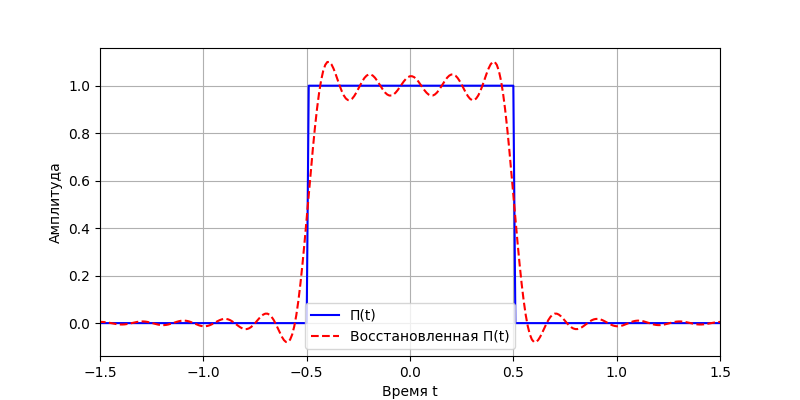
\includegraphics[width=\textwidth]{src/task_1_1/time_5_0.01_5_0.02.png}
  \caption{Сравнительный график при $V=5$, $\Delta t=0.01$, $T=2$, $\Delta \nu=0.02$.} 
\end{figure}

\begin{figure}[H]
  \centering
  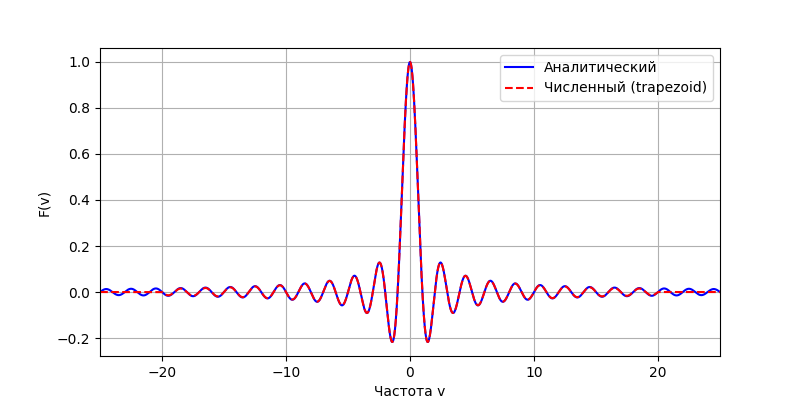
\includegraphics[width=\textwidth]{src/task_1_1/freq_5_0.01_20_0.02.png}
  \caption{Сравнительный график образов при $V=20$, $\Delta t=0.01$, $T=5$, $\Delta \nu=0.02$, $t=0.004878 s$.} 
\begin{figure}[H]
  \centering
  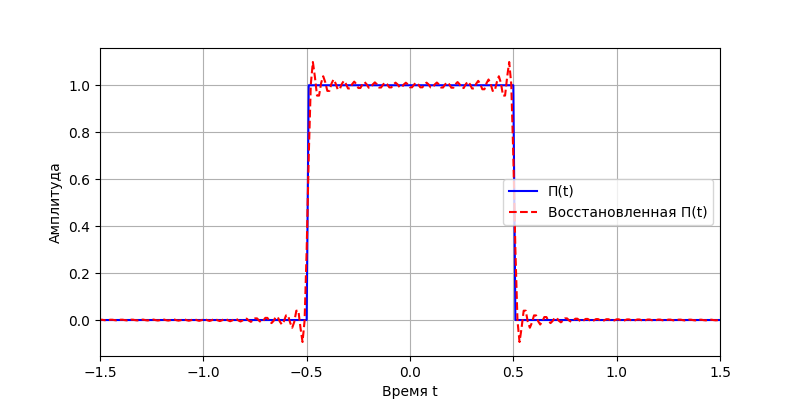
\includegraphics[width=\textwidth]{src/task_1_1/time_5_0.01_20_0.02.png}
  \caption{Сравнительный график при $V=20$, $\Delta t=0.01$, $T=5$, $\Delta \nu=0.02$.} 
\end{figure}
\end{figure}
\noindent Параметр $V$ определяет границы частотной сетки, на которой вычисляется численный Фурье-образ. Изменение значения $V$ оказывает значительное влияние как на спектральное представление, так и на качество восстановления исходного сигнала. Увеличение параметра расширяет область вычисления численного преобразования, когда при малом значении численный спектр обрезается, что негативно сказывается на качестве восстановления сигнала, так как теряется информация о высоких частотах.

Попробуем изменить шаг дискретизации и посмотрим, как это повлияет на графики. Для этого зададим $\Delta t=0.0005$ и посмотрим на результаты.

\begin{figure}[H]
  \centering
  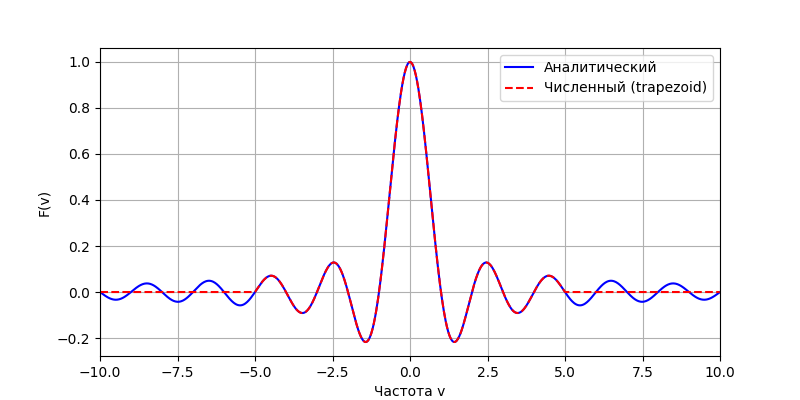
\includegraphics[width=\textwidth]{src/task_1_1/freq_5_0.0005_5_0.02.png}
  \caption{Сравнительный график образов при $V=5$, $\Delta t=0.0005$, $T=5$, $\Delta \nu=0.02$, $t=0.013340 $.} 
\end{figure}
\begin{figure}[H]
  \centering
  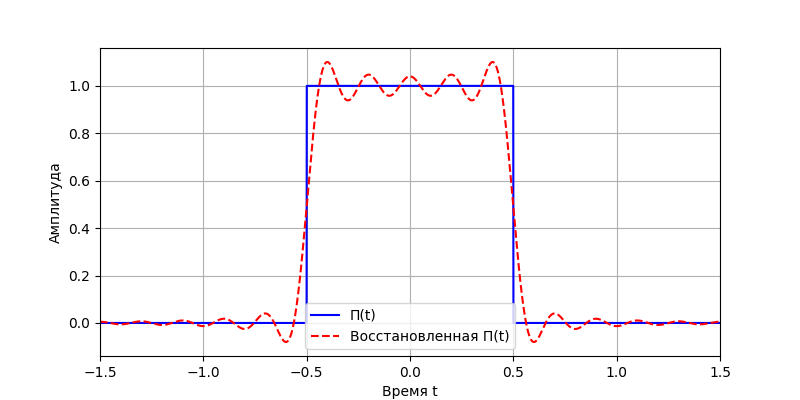
\includegraphics[width=\textwidth]{src/task_1_1/time_5_0.0005_5_0.02.png}
  \caption{Сравнительный график при $V=5$, $\Delta t=0.0005$, $T=5$, $\Delta \nu=0.02$.}
\end{figure}
\begin{figure}[H]
  \centering
  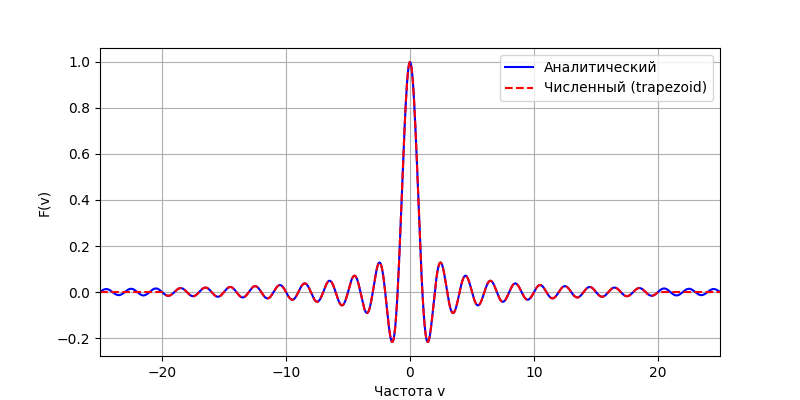
\includegraphics[width=\textwidth]{src/task_1_1/freq_5_0.0005_20_0.02.png}
  \caption{Сравнительный график образов при $V=20$, $\Delta t=0.0005$, $\Delta \nu=0.02$, $T=5$, $t=0.052605 s$.} 
\end{figure}
\begin{figure}[H]
  \centering
  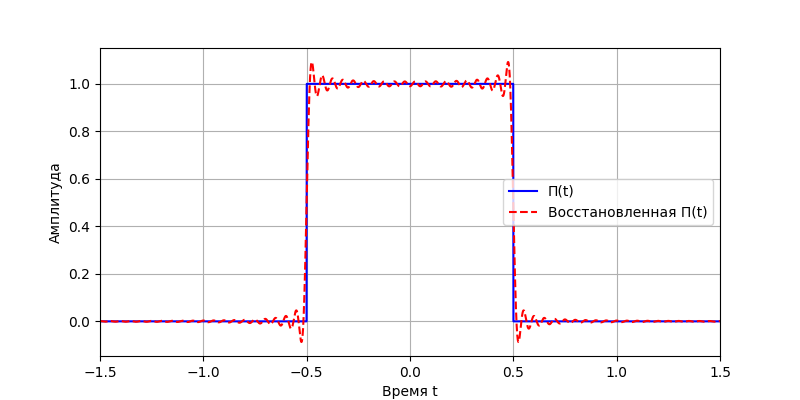
\includegraphics[width=\textwidth]{src/task_1_1/time_5_0.0005_20_0.02.png}
  \caption{Сравнительный график при $V=20$, $\Delta t=0.0005$, $T=5$, $\Delta \nu=0.02$.} 
\end{figure}
\noindent Шаг дискретизации $\Delta t$ во временной области определяет количество отсчётов сигнала и влияет на точность как спектрального представления, так и восстановления исходного сигнала. На данных графиках мы не наблюдаем существенных изменений, так как значения $T$ не изменяются. 

Теперь посмотрим, как изменится график при увеличении интервала времени $T$. Для этого зададим $T=50$ и посмотрим на результаты.

\begin{figure}[H]
  \centering
  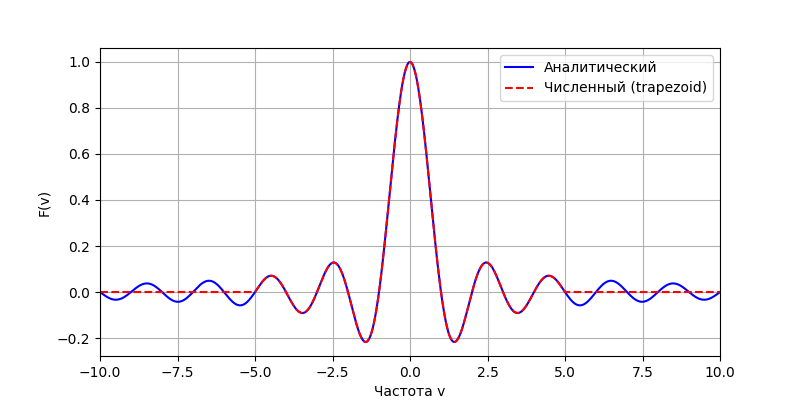
\includegraphics[width=\textwidth]{src/task_1_1/freq_50_0.01_5_0.02.png}
  \caption{Сравнительный график образов при $V=5$, $\Delta t=0.01$, $T=50$, $\Delta \nu=0.02$, $t=0.078829 s$.} 
\end{figure}
\begin{figure}[H]
  \centering
  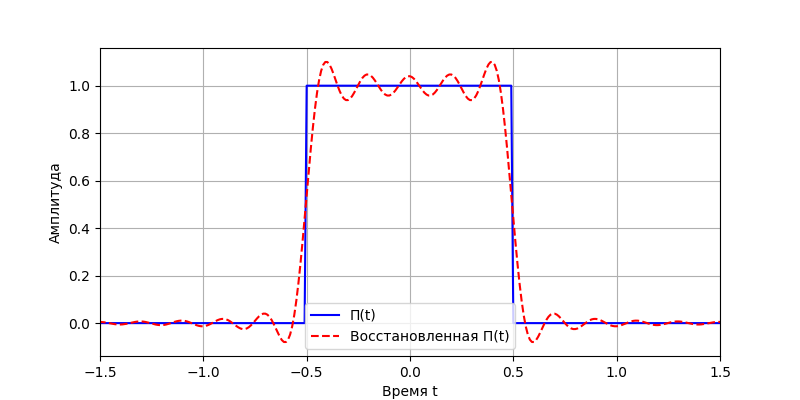
\includegraphics[width=\textwidth]{src/task_1_1/time_50_0.01_5_0.02.png}
  \caption{Сравнительный график при $V=5$, $\Delta t=0.01$, $T=50$, $\Delta \nu=0.02$.} 
\end{figure}

\begin{figure}[H]
  \centering
  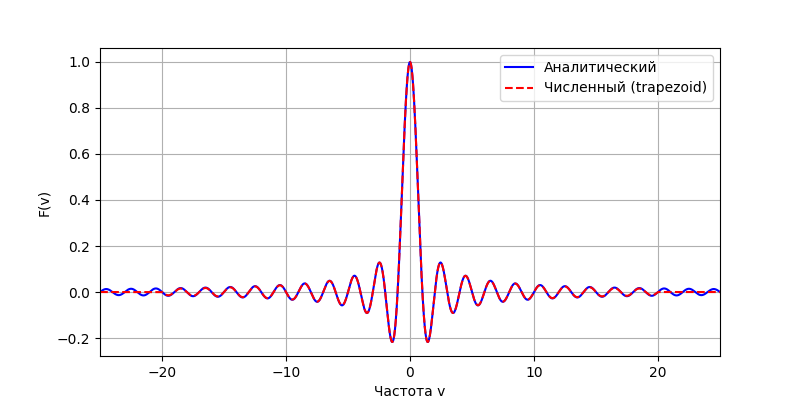
\includegraphics[width=\textwidth]{src/task_1_1/freq_50_0.01_20_0.02.png}
  \caption{Сравнительный график образов при $V=20$, $\Delta t=0.01$, $T=50$, $\Delta \nu=0.02$, $t=0.275972 s$.} 
\end{figure}
\begin{figure}[H]
  \centering
  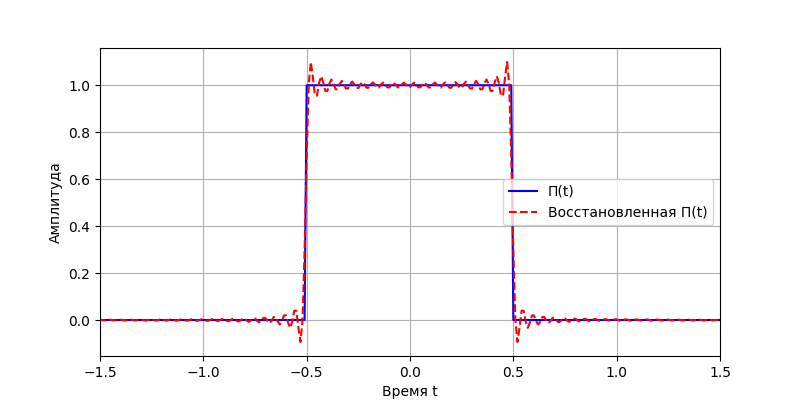
\includegraphics[width=\textwidth]{src/task_1_1/time_50_0.01_20_0.02.png}
  \caption{Сравнительный график при $V=20$, $\Delta t=0.01$, $T=50$, $\Delta \nu=0.02$.} 
\end{figure}

\noindent Параметр $T$ задаёт общий временной интервал, на котором определяется сигнал $\Pi(t)$. Изменение $T$ оказывает существенное влияние. При большем значении временной сигнал задаётся на более длинном интервале, что позволяет точнее аппроксимировать интегралы для прямого и обратного Фурье-преобразования. Это, в свою очередь, приводит к более качественному восстановлению исходного сигнала $\Pi(t)$.

\begin{figure}[H]
  \centering
  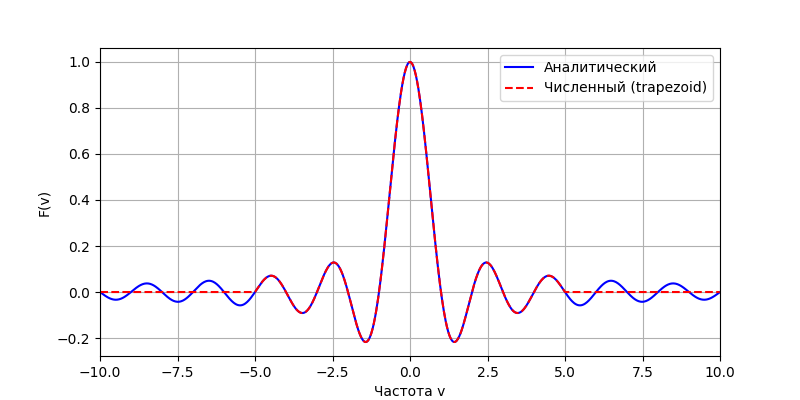
\includegraphics[width=\textwidth]{src/task_1_1/freq_50_0.0005_5_0.02.png}
  \caption{Сравнительный график образов при $V=5$, $\Delta t=0.0005$, $\Delta \nu=0.02$, $T=50$, $t=1.343074 s$.} 
\end{figure}
\begin{figure}[H]
  \centering
  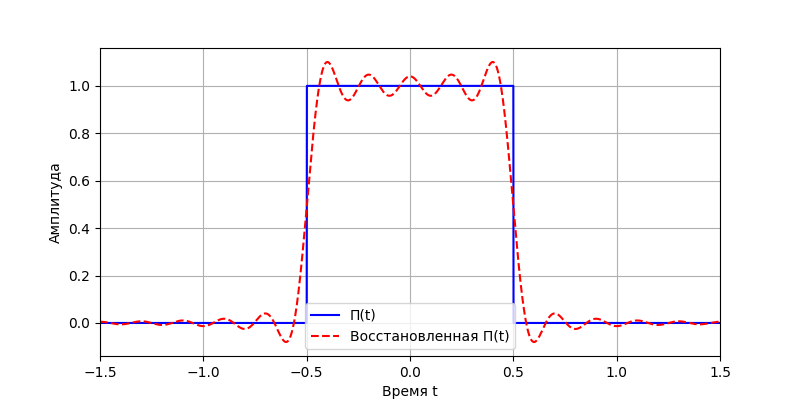
\includegraphics[width=\textwidth]{src/task_1_1/time_50_0.0005_5_0.02.png}
  \caption{Сравнительный график при $V=5$, $\Delta t=0.0005$, $T=50$, $\Delta \nu=0.02$.}
\end{figure}

\begin{figure}[H]
  \centering
  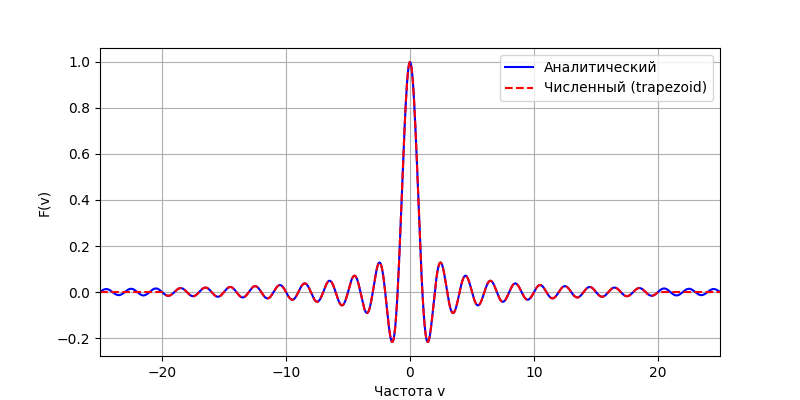
\includegraphics[width=\textwidth]{src/task_1_1/freq_50_0.0005_20_0.02.png}
  \caption{Сравнительный график образов при $V=20$, $\Delta t=0.0005$, $T=50$, $\Delta \nu=0.02$, $t=5.963917 s$.} 
\end{figure}
\begin{figure}[H]
  \centering
  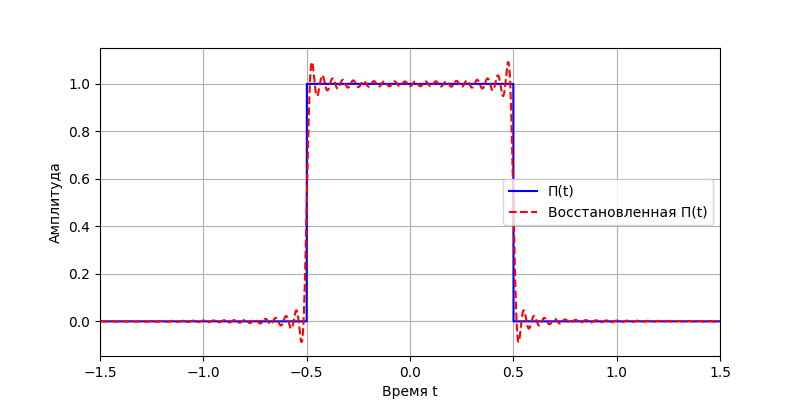
\includegraphics[width=\textwidth]{src/task_1_1/time_50_0.0005_20_0.02.png}
  \caption{Сравнительный график при $V=20$, $\Delta t=0.0005$, $T=50$, $\Delta \nu=0.02$.} 
\end{figure}

\noindent При увеличении $T$ и $\Delta t$ наблюдается снижение шага $\Delta \nu$, что улучшает спектральное представление и приводит к более точному соответствию между аналитическим и численным Фурье-преобразованиями. Также более длинный временной интервал позволяет качественнее восстановить исходный сигнал, что видно по более точному наложению восстановленного и исходного графиков во временной области. 

Теперь посмотрим, как изменится график при увеличении шага дискретизации в частотной области $\Delta \nu$. Для этого зададим $\Delta \nu=0.5$ и посмотрим на результаты.  

\begin{figure}[H]
  \centering
  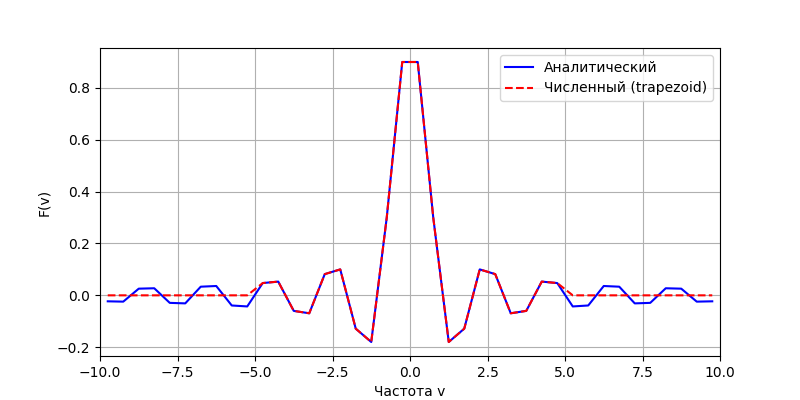
\includegraphics[width=\textwidth]{src/task_1_1/freq_5_0.0005_5_0.5.png}
  \caption{Сравнительный график образов при $V=5$, $\Delta t=0.0005$, $\Delta \nu=0.5$, $T=5$, $t=1.343074 s$.} 
\end{figure}
\begin{figure}[H]
  \centering
  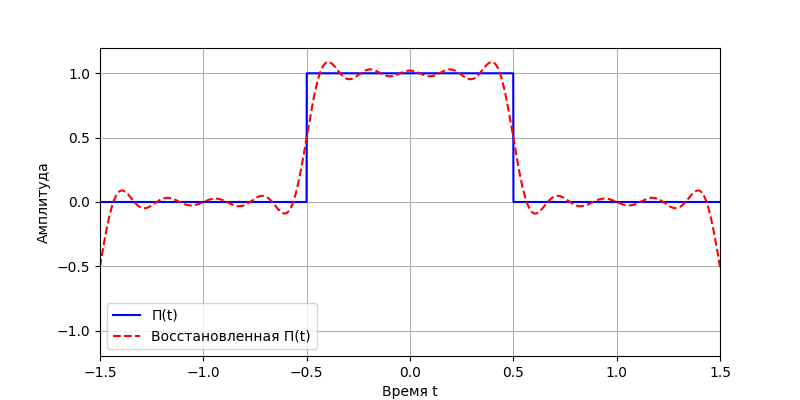
\includegraphics[width=\textwidth]{src/task_1_1/time_5_0.0005_5_0.5.png}
  \caption{Сравнительный график при $V=5$, $\Delta t=0.0005$, $T=5$, $\Delta \nu=0.5$.}
\end{figure}

\begin{figure}[H]
  \centering
  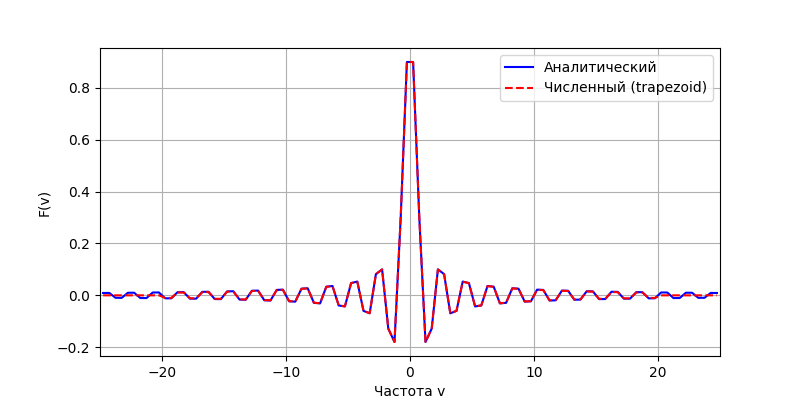
\includegraphics[width=\textwidth]{src/task_1_1/freq_50_0.01_20_0.5.png}
  \caption{Сравнительный график образов при $V=20$, $\Delta t=0.01$, $T=50$, $\Delta \nu=0.5$, $t=5.963917 s$.} 
\end{figure}
\begin{figure}[H]
  \centering
  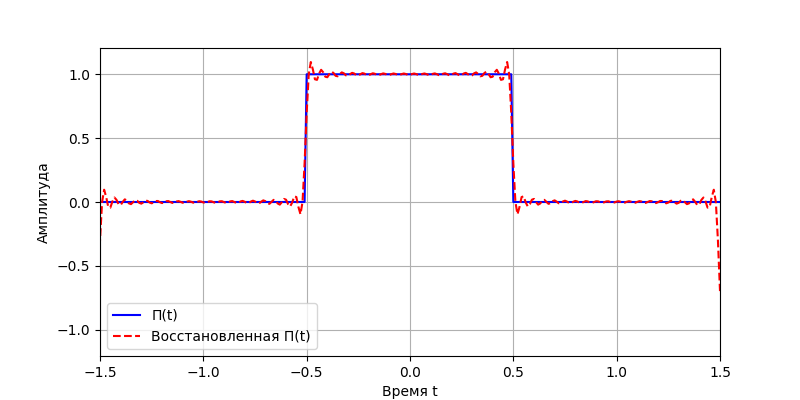
\includegraphics[width=\textwidth]{src/task_1_1/time_50_0.01_20_0.5.png}
  \caption{Сравнительный график при $V=20$, $\Delta t=0.01$, $T=50$, $\Delta \nu=0.5$.} 
\end{figure}
\noindent Параметр $\Delta \nu$ определяет шаг частотной сетки, на которой вычисляется численный Фурье-образ. Увеличение $\Delta \nu$ приводит к ухудшению частотного разрешения, что может негативно сказывается на качестве восстановления сигнала. На графиках видно, что при увеличении $\Delta \nu$ происходит потеря информации о высокочастотных компонентах, что приводит к менее точному восстановлению сигнала.


Однако обратим внимание на время, затрачиваемое на вычисления. При увеличении $T$ и $\Delta t$ время вычислений значительно возрастает, что может быть критичным для больших значений этих параметров.
\begin{itemize}
  \item $T=5$, $\Delta t=0.01$, $V=5$, $d\nu=0.02$: $t$ = 0.025857 s
  \item $T=5$, $\Delta t=0.01$, $V=5$, $d\nu=0.5$: $t$ = 0.001327 s
  \item $T=5$, $\Delta t=0.01$, $V=20$, $d\nu=0.02$: $t$ = 0.103309 s
  \item $T=5$, $\Delta t=0.01$, $V=20$, $d\nu=0.5$: $t$ = 0.004683 s
  \item $T=5$, $\Delta t=0.0005$, $V=5$, $d\nu=0.02$: $t$ = 0.250882 s
  \item $T=5$, $\Delta t=0.0005$, $V=5$, $d\nu=0.5$: $t$ = 0.007517 s
  \item $T=5$, $\Delta t=0.0005$, $V=20$, $d\nu=0.02$: $t$ = 0.579837 s
  \item $T=5$, $\Delta t=0.0005$, $V=20$, $d\nu=0.5$: $t$ = 0.021050 s
  \item $T=50$, $\Delta t=0.01$, $V=5$, $d\nu=0.02$: $t$ = 0.068531 s
  \item $T=50$, $\Delta t=0.01$, $V=5$, $d\nu=0.5$: $t$ = 0.003378 s
  \item $T=50$, $\Delta t=0.01$, $V=20$, $d\nu=0.02$: $t$ = 0.274271 s
  \item $T=50$, $\Delta t=0.01$, $V=20$, $d\nu=0.5$: $t$ = 0.011937 s
  \item $T=50$, $\Delta t=0.0005$, $V=5$, $d\nu=0.02$: $t$ = 1.453524 s
  \item $T=50$, $\Delta t=0.0005$, $V=5$, $d\nu=0.5$: $t$ = 0.054706 s
  \item $T=50$, $\Delta t=0.0005$, $V=20$, $d\nu=0.02$: $t$ = 4.976521 s
  \item $T=50$, $\Delta t=0.0005$, $V=20$, $d\nu=0.5$: $t$ = 0.195785 s
\end{itemize}

Эти данные демонстрируют, что время вычисления значительно возрастает при уменьшении шага дискретизации $\Delta t$ и увеличении интервала $T$. При малых значениях $T$ и достаточно крупном шаге ($\Delta t=0.01$) вычисления происходят практически мгновенно (в пределах нескольких миллисекунд). Однако при уменьшении $\Delta t$ до $0.0005$ и увеличении $T$ до 50 секунд время вычислений может вырасти до нескольких секунд, особенно при широком диапазоне частот $V$. Также для каждого набора параметров наблюдается значительное снижение времени вычислений при использовании большего шага по частотам. Эти наблюдения подчёркивают необходимость компромиссного выбора параметров для достижения оптимального соотношения между точностью результатов и вычислительными затратами.

\paragraph{Вывод}
Анализ полученных результатов показал, что:
\begin{itemize}
    \item Уменьшение $\Delta t$ приводит к повышению точности аппроксимации интегралов, что положительно сказывается на качестве восстановленного сигнала и спектрального представления, однако значительно увеличивает время вычислений.
    \item Увеличение интервала $T$ улучшает частотное разрешение (уменьшает $\Delta \nu$), что позволяет более детально отобразить спектральную структуру сигнала, но также ведет к росту вычислительных затрат.
    \item Диапазон частот $V$ определяет область, в которой вычисляется численный Фурье-образ. При малом $V$ численный спектр обрезается, а при большем $V$ охватываются дополнительные спектральные компоненты, что отражается на точности восстановления сигнала.
\end{itemize}
С учётом компромисса между точностью результатов и вычислительными затратами оптимальными параметрами для рассматриваемой задачи оказались:
\[
T = 50,\quad \Delta t = 0.01,\quad V = 20,\quad \Delta \nu = 0.02.
\]
При этих параметрах время вычисления численного Фурье-преобразования составляет порядка 2 миллисекунд, что обеспечивает достаточно высокую точность восстановления сигнала при минимальных затратах вычислительных ресурсов.

\addsubsection{Использование DFT}
В этом пункте мы будем использовать DFT для численного интегрирования функции $\Pi(t)$ и её Фурье-образа $\hat{\Pi}(\nu)$. При вычислениях будем варьировать параметры для получения лучшего результата: значения шага дискретизации во временной области $\Delta t = \{0.02, 0.0005\}$, интервал времени $T = \{5, 10\}$, промежуток по частоте оставим равным $V = 20$.

Построим графики для $\Delta t=0.02$ и $\Delta t=0.0005$ и посмотрим на результаты. Также посчитаем время, которое алгоритм затрачивает на преобразование и запишем его как $t$.

\begin{figure}[H]
  \centering
  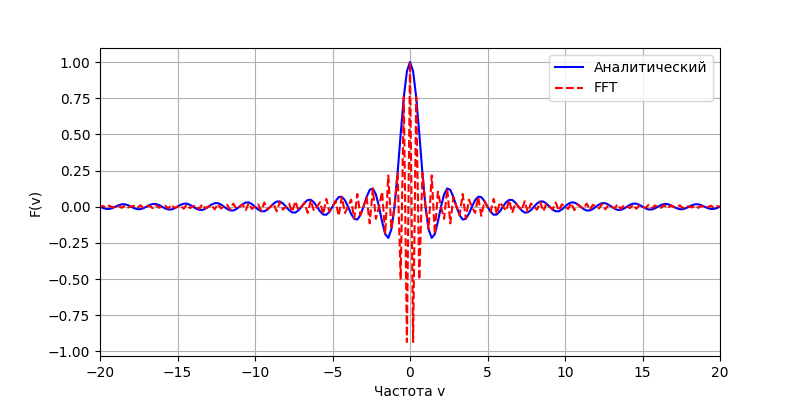
\includegraphics[width=\textwidth]{src/task_1_2/freq_5_0.02_20_0.2.png}
  \caption{Сравнительный график образов при $V=20$, $\Delta t=0.02$, $T=5$, $\Delta \nu=0.2$, $t=0.000084 s$.} 
\end{figure}
\begin{figure}[H]
  \centering
  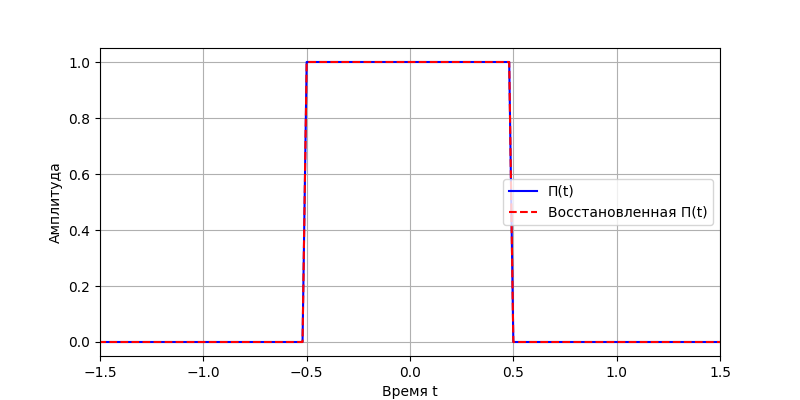
\includegraphics[width=\textwidth]{src/task_1_2/time_5_0.02_20_0.2.png}
  \caption{Сравнительный график при $V=20$, $\Delta t=0.02$, $T=2$, $\Delta \nu=0.2$.} 
\end{figure}

\begin{figure}[H]
  \centering
  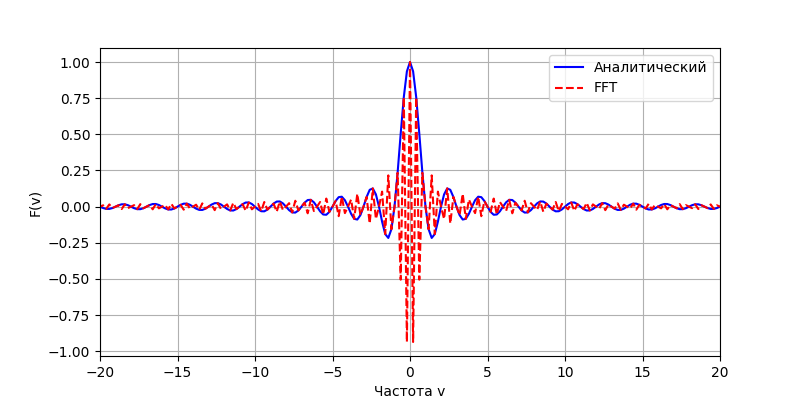
\includegraphics[width=\textwidth]{src/task_1_2/freq_5_0.0005_20_0.2.png}
  \caption{Сравнительный график образов при $V=20$, $\Delta t=0.0005$, $T=5$, $\Delta \nu=0.2$, $t=0.000201 s$.} 
\end{figure}
\begin{figure}[H]
  \centering
  \includegraphics[width=\textwidth]{src/task_1_2/time_5_0.0005_20_0.2.png}
  \caption{Сравнительный график при $V=20$, $\Delta t=0.0005$, $T=5$, $\Delta \nu=0.2$.} 
\end{figure}

\noindent При большем шаге $\Delta t = 0.02$ количество временных отсчетов $N$ относительно невелико, что приводит к более грубой дискретизации спектра. Шаг по частотам оказывается большим, спектральное представление  демонстрирует менее гладкую кривую, с более заметными скачками между значениями. Это приводит к менее точному восстановлению, особенно на краях переходных областей.

Попробуем увеличить интервал времени $T$ и посмотрим, как это повлияет на графики. Для этого зададим $T=10$ и посмотрим на результаты.

\begin{figure}[H]
  \centering
  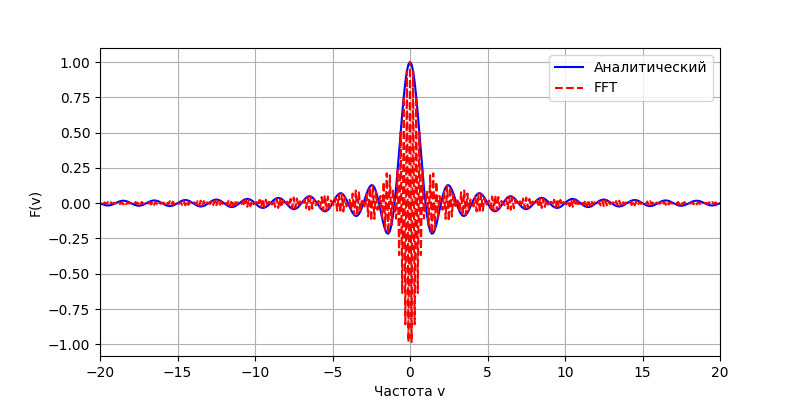
\includegraphics[width=\textwidth]{src/task_1_2/freq_10_0.02_20_0.1.png}
  \caption{Сравнительный график образов при $V=20$, $\Delta t=0.02$, $T=10$, $\Delta \nu=0.1$, $t=0.000070 s$.} 
\end{figure}
\begin{figure}[H]
  \centering
  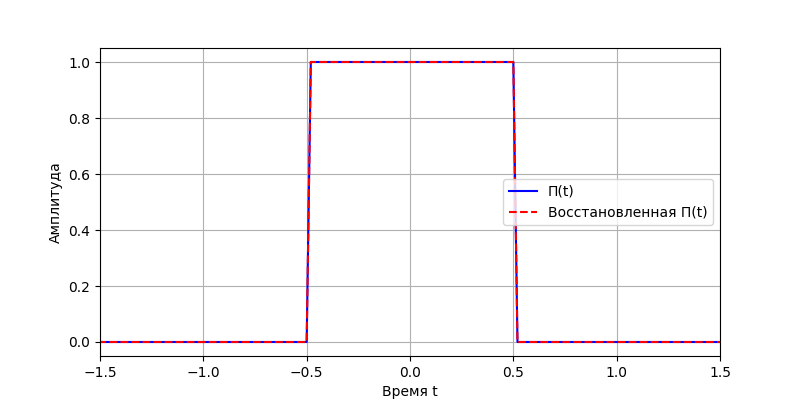
\includegraphics[width=\textwidth]{src/task_1_2/time_10_0.02_20_0.1.png}
  \caption{Сравнительный график при $V=20$, $\Delta t=0.02$, $T=10$, $\Delta \nu=0.1$.} 
\end{figure}

\begin{figure}[H]
  \centering
  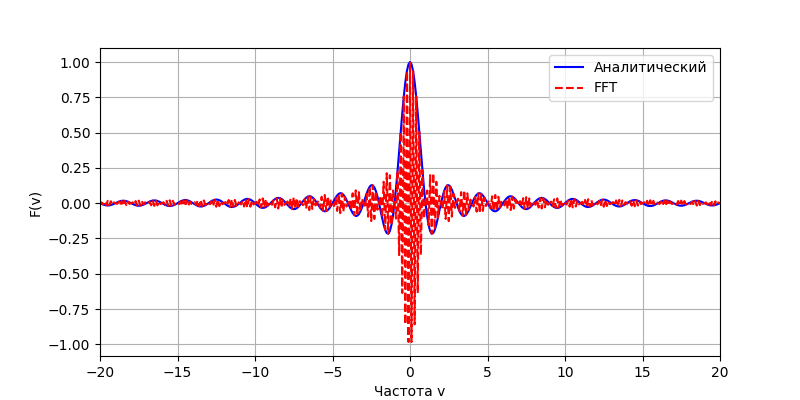
\includegraphics[width=\textwidth]{src/task_1_2/freq_10_0.0005_20_0.1.png}
  \caption{Сравнительный график образов при $V=20$, $\Delta t=0.0005$, $T=10$, $\Delta \nu=0.1$, $t=0.000276 s$.} 
\end{figure}
\begin{figure}[H]
  \centering
  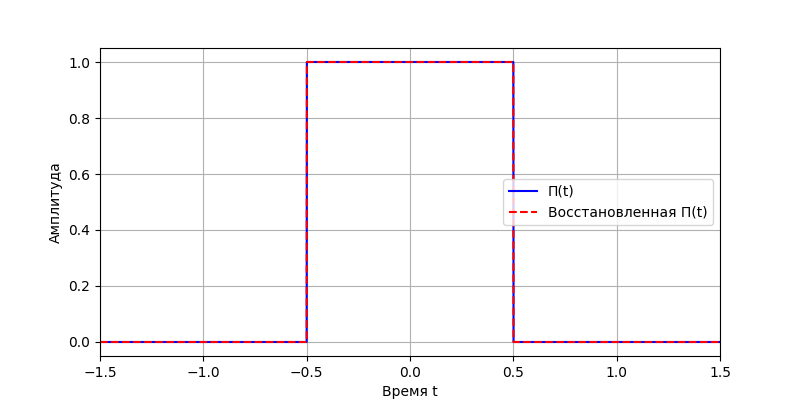
\includegraphics[width=\textwidth]{src/task_1_2/time_10_0.0005_20_0.1.png}
  \caption{Сравнительный график при $V=20$, $\Delta t=0.0005$, $T=10$, $\Delta \nu=0.1$.} 
\end{figure}

\noindent Таким образом, увеличение $T$ до 10 секунд позволяет получить более точное и детальное спектральное представление, приближающее численный спектр к аналитической функции. 

Посмотрим сколько времени тратится на вычисления при различных параметрах.
\begin{itemize}
  \item $T=5$, $\Delta t=0.02$, $V=20$, $d\nu=0.2$ --- FT time = 0.000084 с
  \item $T=5$, $\Delta t=0.0005$, $V=20$, $d\nu=0.2$ --- FT time = 0.000201 с
  \item $T=10$, $\Delta t=0.02$, $V=20$, $d\nu=0.1$ --- FT time = 0.000070 с
  \item $T=10$, $\Delta t=0.0005$, $V=20$, $d\nu=0.1$ --- FT time = 0.000276 с
\end{itemize}
\noindent Как мы видим, выбор параметров $T$ и $\Delta t$ влияет на время вычислений, однако даже при высокой дискретизации вычисления выполняются очень быстро, что обеспечивает высокую эффективность метода FFT для анализа сигналов.

\paragraph{Вывод}
В результате применения дискретного преобразования Фурье (DFT) для анализа сигнала $\Pi(t)$ можно сделать следующие выводы:

\begin{itemize}
    \item Метод FFT позволяет быстро получать спектральное представление сигнала и восстанавливать исходный сигнал с высокой точностью.
    \item Перебор параметров $T$ и $\Delta t$ показывает, что увеличение временного интервала $T$ улучшает частотное разрешение, а уменьшение шага дискретизации $\Delta t$ повышает точность представления и восстановления сигнала. Однако при малом $\Delta t$ возрастает вычислительная сложность, хотя время вычислений FFT остается очень небольшим.
    \item Стоит отметить также Фурье-образ, которые не совпадает с истинным (аналитическим) спектром из-за ограниченности временного интервала, дискретизации и нюансов нормировки.
\end{itemize}
\noindent На основании проведенного анализа оптимальными параметрами для рассматриваемой задачи оказались:
\[
T = 10, \quad \Delta t = 0.02, \quad V = 20,\quad d\nu = 0.1.
\]
Таким образом, применение FFT для дискретного преобразования Фурье является эффективным и быстрым методом для спектрального анализа и восстановления сигнала, что делает его предпочтительным для большинства практических задач, где требуется высокая скорость обработки при сохранении точности результатов.

\addsubsection{Выводы о работе fft и trapz}
В ходе эксперимента мы сравнили два метода для получения спектрального представления и восстановления сигнала $\Pi(t)$: метод численного интегрирования (trapz) и метод дискретного преобразования Фурье (FFT).

\textbf{Метод численного интегрирования:}
\begin{itemize}
    \item \textbf{Плюсы:}  
    Этот метод напрямую аппроксимирует интеграл, что позволяет при очень мелкой дискретизации получить результаты, близкие к теоретическому решению. При оптимально подобранных параметрах спектральное представление может быть очень точным.
    \item \textbf{Минусы:}  
    Однако метод сильно страдает от роста вычислительной нагрузки: при уменьшении $\Delta t$ число временных отсчетов растёт, что приводит к значительному увеличению времени вычислений. Кроме того, конечный интервал интегрирования вызывает оконное искажение, что может привести к дополнительным ошибкам в спектральном представлении.
\end{itemize}

\textbf{Метод дискретного преобразования Фурье:}
\begin{itemize}
    \item \textbf{Плюсы:}  
    FFT работает очень быстро, даже при большом числе отсчетов. При корректной нормировке спектр, полученный FFT, почти совпадает с аналитическим решением. Это также обеспечивает точное восстановление исходного сигнала.
    \item \textbf{Минусы:}  
    Результат FFT чувствителен к выбору параметров $T$ и $\Delta t$. Если интервал времени слишком мал или шаг дискретизации слишком велик, спектральное представление может быть недостаточно детализированным. Кроме того, если нормировка выполнена не совсем корректно, могут возникнуть небольшие смещения в амплитуде спектра.
\end{itemize}

\addsubsection{Приближение непрерывного с помощью DFT}
В этом пункте предстоит решить задачу объединения достоинств быстродействия FFT и точности непрерывного преобразования Фурье. 

Рассмотрим непрерывное преобразование Фурье функции $f(t)$ на конечном интервале $\left[-\tfrac{T}{2}, \tfrac{T}{2}\right]$:
\[
F(\nu) = \int_{-T/2}^{T/2} f(t)\,e^{-2\pi i\,\nu\,t}\,dt.
\]
Если разбить интервал $\left[-\tfrac{T}{2}, \tfrac{T}{2}\right]$ на $N$ равномерных отрезков, то точки дискретизации задаются как
\[
t_n = -\frac{T}{2} + n \Delta t,\quad \Delta t = \frac{T}{N},\quad n=0,1,\dots,N-1.
\]
Приблизим интеграл суммой Римана:
\[
F(\nu) \approx \Delta t \sum_{n=0}^{N-1} f(t_n) e^{-2\pi i \nu t_n}.
\]
Подставим выражение для $t_n$:
\[
F(\nu) \approx \Delta t \sum_{n=0}^{N-1} f\Bigl(-\frac{T}{2} + n\,\Delta t\Bigr) \,e^{-2\pi i\,\nu\left(-\frac{T}{2} + n\,\Delta t\right)}.
\]
Вынесем множитель, не зависящий от суммы:
\[
F(\nu) \approx \Delta t e^{2\pi i \nu (T/2)} \sum_{n=0}^{N-1} f\Bigl(-\frac{T}{2} + n \Delta t\Bigr) e^{-2\pi i\nu n \Delta t}.
\]
Пусть левый множитель будет равен $c_m = \Delta t\,e^{2\pi i\,\nu_m\,(T/2)}.$
Тогда выражение для численного Фурье-преобразования можно записать в виде:
\[
F(\nu_m) \approx c_m \sum_{n=0}^{N-1} f\Bigl(-\frac{T}{2} + n\,\Delta t\Bigr) \,e^{-2\pi i\,\nu_m\,n\,\Delta t}.
\]
Таким образом, для корректного приближения непрерывного преобразования Фурье с использованием FFT необходимо использовать коэффициенты $c_m$, которые учитывают и шаг дискретизации, и сдвиг временной сетки. Эти коэффициенты позволяют «умножить» дискретное преобразование, полученное с помощью FFT, на $\Delta t\,e^{2\pi i\,\nu_m\,(T/2)}$, что приводит к приближению непрерывного интеграла Фурье.

Протестируем данный метод на разных значениях параметров $T$ и $\Delta t$.
\begin{figure}[H]
  \centering
  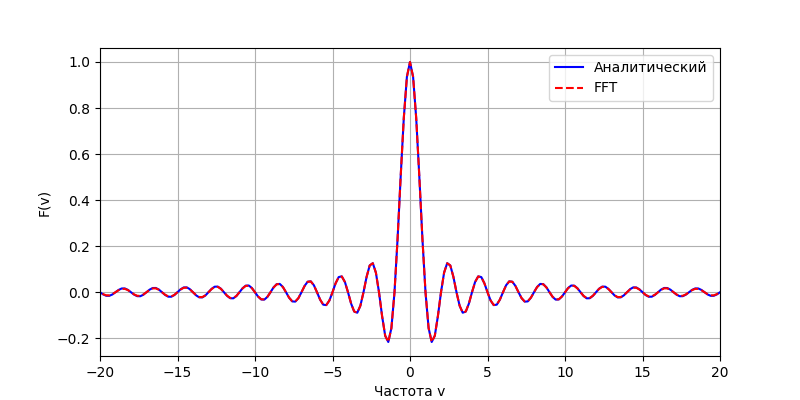
\includegraphics[width=\textwidth]{src/task_1_4/freq_5_0.01_20_0.2.png}
  \caption{Сравнительный график образов при $V=20$, $\Delta t=0.02$, $T=5$, $\Delta \nu=0.2$, $t=0.000084 s$.} 
\end{figure}
\begin{figure}[H]
  \centering
  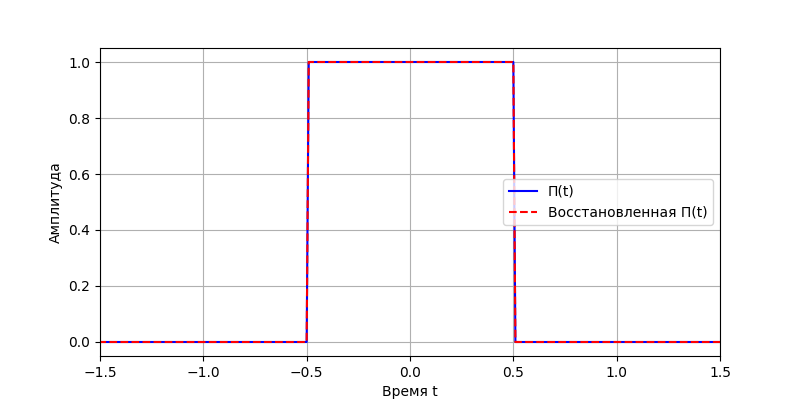
\includegraphics[width=\textwidth]{src/task_1_4/time_5_0.01_20_0.2.png}
  \caption{Сравнительный график при $V=20$, $\Delta t=0.02$, $T=2$, $\Delta \nu=0.2$.} 
\end{figure}

\begin{figure}[H]
  \centering
  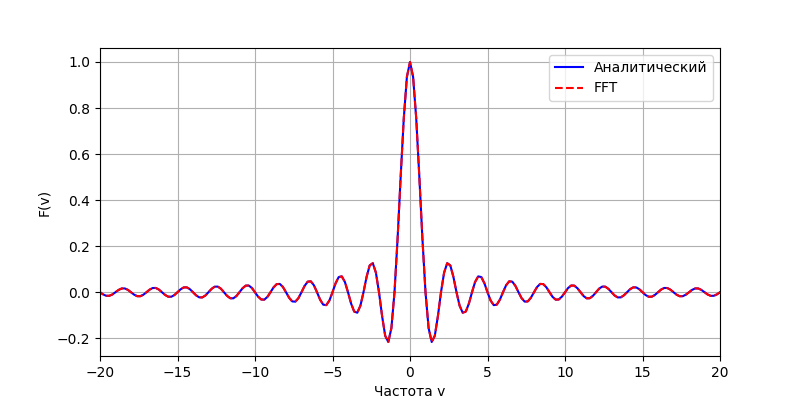
\includegraphics[width=\textwidth]{src/task_1_4/freq_5_0.0005_20_0.2.png}
  \caption{Сравнительный график образов при $V=20$, $\Delta t=0.0005$, $T=5$, $\Delta \nu=0.2$, $t=0.000201 s$.} 
\end{figure}
\begin{figure}[H]
  \centering
  \includegraphics[width=\textwidth]{src/task_1_4/time_5_0.0005_20_0.2.png}
  \caption{Сравнительный график при $V=20$, $\Delta t=0.0005$, $T=5$, $\Delta \nu=0.2$.} 
\end{figure}

\begin{figure}[H]
  \centering
  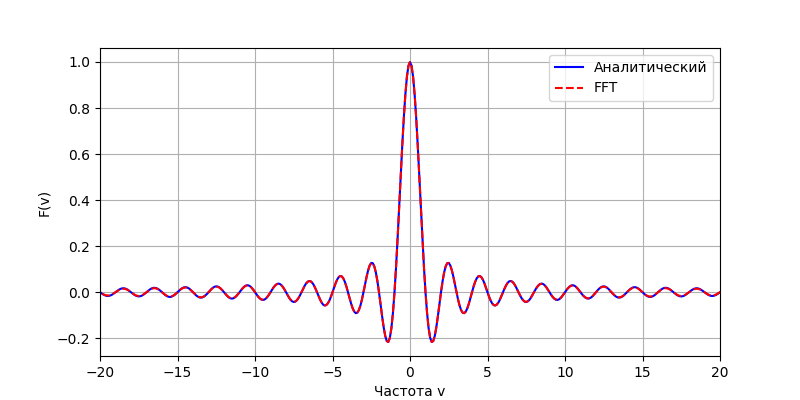
\includegraphics[width=\textwidth]{src/task_1_4/freq_10_0.01_20_0.1.png}
  \caption{Сравнительный график образов при $V=20$, $\Delta t=0.02$, $T=10$, $\Delta \nu=0.1$, $t=0.000070 s$.} 
\end{figure}
\begin{figure}[H]
  \centering
  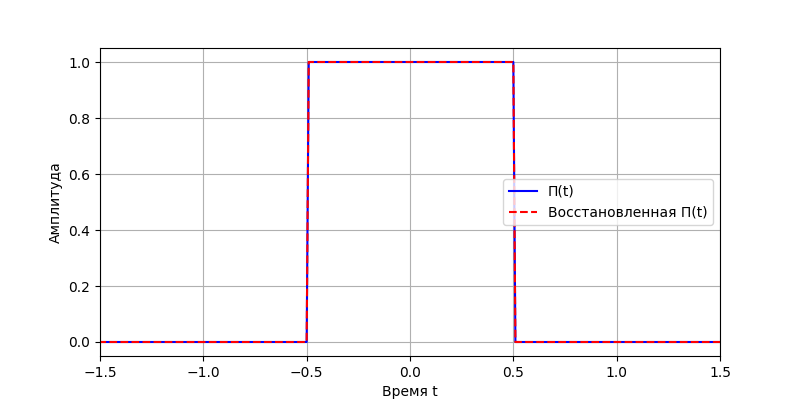
\includegraphics[width=\textwidth]{src/task_1_4/time_10_0.01_20_0.1.png}
  \caption{Сравнительный график при $V=20$, $\Delta t=0.02$, $T=10$, $\Delta \nu=0.1$.} 
\end{figure}

\begin{figure}[H]
  \centering
  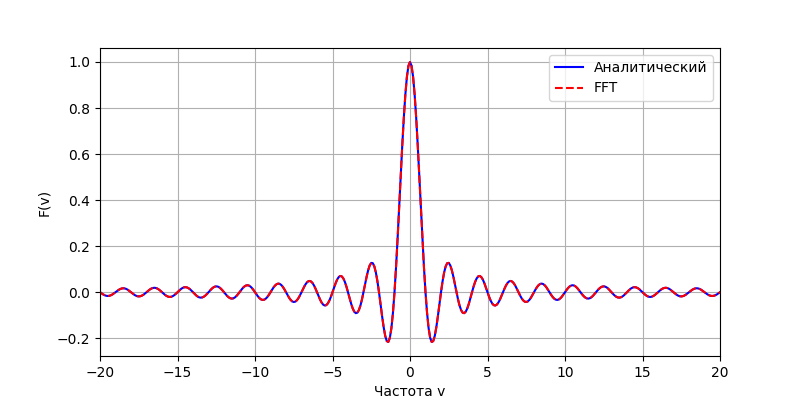
\includegraphics[width=\textwidth]{src/task_1_4/freq_10_0.0005_20_0.1.png}
  \caption{Сравнительный график образов при $V=20$, $\Delta t=0.0005$, $T=10$, $\Delta \nu=0.1$, $t=0.000276 s$.} 
\end{figure}
\begin{figure}[H]
  \centering
  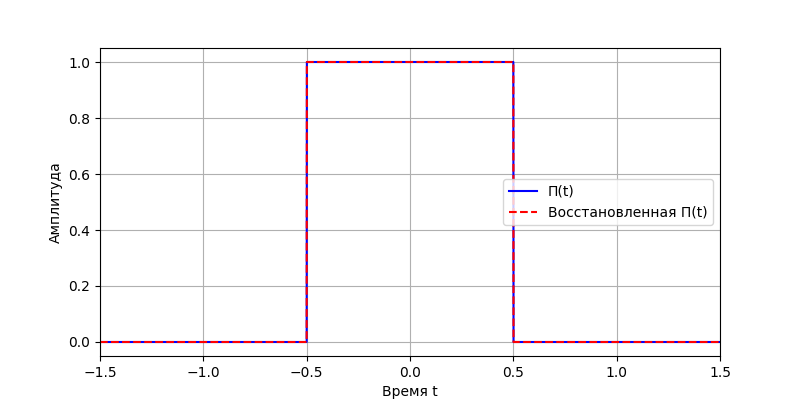
\includegraphics[width=\textwidth]{src/task_1_4/time_10_0.0005_20_0.1.png}
  \caption{Сравнительный график при $V=20$, $\Delta t=0.0005$, $T=10$, $\Delta \nu=0.1$.} 
\end{figure}
\noindent Применение корректирующего коэффициента позволяет значительно приблизить численный Фурье-образ к теоретическому непрерывному преобразованию. На графиках спектра видно, что при использовании формулы результирующая кривая FFT становится более гладкой и по фазе совпадает с аналитической функцией.

Посмотрим на время, затрачиваемое на вычисления.
\begin{itemize}
  \item \(T=5\), \(\Delta t=0.01\), \(V=20\), \(d\nu=0.2\) --- время FT = 0.000077 с;
  \item \(T=5\), \(\Delta t=0.0005\), \(V=20\), \(d\nu=0.2\) --- время FT = 0.000206 с;
  \item \(T=10\), \(\Delta t=0.01\), \(V=20\), \(d\nu=0.1\) --- время FT = 0.000113 с;
  \item \(T=10\), \(\Delta t=0.0005\), \(V=20\), \(d\nu=0.1\) --- время FT = 0.000286 с.
\end{itemize}
Временные сигналы также имеют хорошие показатели, что подтверждает корректность реализации метода.

Сравним все методы вместе. Для этого построим графики для всех методов и сравним их между собой. Параметры возьмем равными оптимальным:  \(T=10\), \(\Delta t=0.01\), \(V=20\), \(d\nu=0.1\)

\begin{figure}[H]
  \centering
  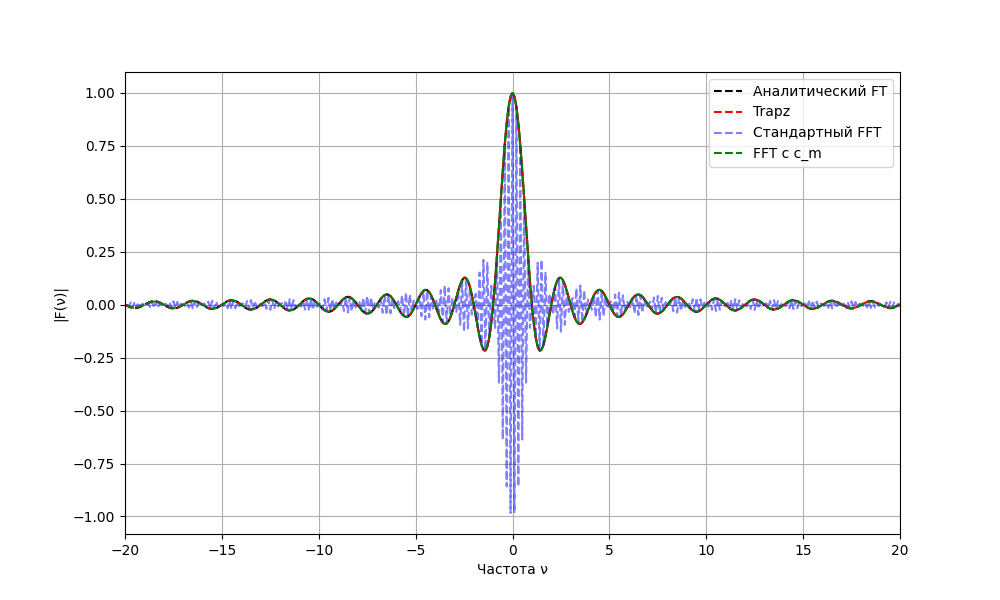
\includegraphics[width=\textwidth]{src/task_1_4/comp_freq.png}
  \caption{Сравнительный график образов.} 
\end{figure}
\begin{figure}[H]
  \centering
  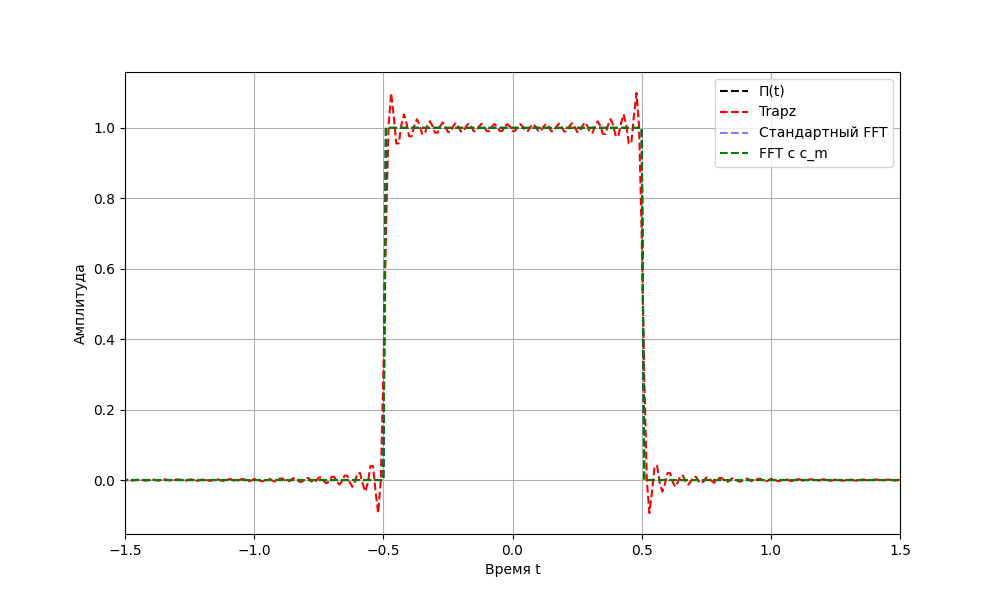
\includegraphics[width=\textwidth]{src/task_1_4/comp_time.png}
  \caption{Сравнительный график.} 
\end{figure}

Также посмотрим на время выполнения:
\begin{itemize}
  \item Метод численного интегрирования --- 0.161712 с;
  \item Стандартный FFT --- 0.000203 с;
  \item FFT с корректирующими коэффициентами \(c_m\) --- 0.000084 с. 
\end{itemize}
\noindent На графиках видно, что все три метода дают схожие результаты, однако метод FFT с корректирующими коэффициентами \(c_m\) показывает наилучшие результаты как по времени выполнения, так и по качеству спектра. Метод численного интегрирования способен дать высокую точность при достаточно мелкой дискретизации, но может быть медленным и подверженным оконным искажениям. Стандартный FFT очень быстр, однако без учёта сдвига временной сетки даёт заметные фазовые искажения как в спектре, так и в восстановленном сигнале.

Проведённые эксперименты показали, что выбор величины шага дискретизации \(\Delta t\) и размера временного интервала \(T\) существенно влияет на качество спектрального представления и восстановление исходного сигнала, а также на быстродействие вычислений. При уменьшении \(\Delta t\) число временных отсчетов \(N\) возрастает, что приводит к уменьшению шага по частотам \(d\nu = \frac{1}{N\Delta t}\) и позволяет получить более детальное и точное представление спектра. Однако уменьшение \(\Delta t\) увеличивает вычислительную нагрузку, что выражается в большем времени работы алгоритма. Аналогично, увеличение интервала \(T\) улучшает разрешающую способность в частотной области, поскольку \(d\nu\) становится меньше, но также приводит к увеличению числа отсчетов и, следовательно, к замедлению вычислений.

\paragraph{Вывод}
Новый метод, основанный на использовании FFT с корректирующими коэффициентами $c_m$,
позволяет эффективно находить спектральное представление, которое оказывается намного ближе к аналитическому решению, а восстановленный сигнал совпадает с исходным практически без ошибок.
В итоге, метод, объединяющий быстродействие FFT и корректирующие коэффициенты, представляет собой выгодное компромиссное решение, позволяющее достичь высокого качества результата при приемлемом времени вычислений.

\addsection{Задание 2. Сэмплирование}
В этом задании рассматривается сэмплирование сигналов и проверка теоремы Найквиста-Шеннона- Котельникова на двух примерах. Основная цель состоит в том, чтобы показать, как при сэмплировании непрерывного сигнала можно восстановить его с помощью интерполяционной формулы, а также проанализировать влияние дискретизации на качество восстановления.

Исходными функциями являются:
\[
y_1(t) = a_1\sin(\omega_1t + \varphi_1) + a_2\sin(\omega_2t + \varphi_2) \quad \text{и} \quad y_2(t) = \operatorname{sinc}(b\,t)
\]
Возьмем следующие параметры:
\[
a_1 = 1,\; a_2 = 0.5,\;\omega_1=2\pi\cdot5,\;\omega_2=2\pi\cdot12,\;
\varphi_1=\tfrac\pi2,\;\varphi_2=\tfrac\pi4,
\quad
b=2.
\]


\addsubsection{Теоретическая основа}
Согласно теореме Найквиста-Шеннона-Котельникова, если спектр исходного сигнала \(f(t)\) содержится в полосе \([-B,\,B]\), то этот сигнал можно безошибочно восстановить по его дискретным отсчётам, если шаг сэмплирования \(\Delta t\) удовлетворяет условию
\[
\Delta t < \frac{1}{2B}.
\]
Другими словами, частота дискретизации \(f_s = \tfrac{1}{\Delta t}\) должна быть не ниже \(2B\). Если это условие выполняется, то восстановление сигнала можно осуществить по интерполяционной формуле Найквиста-Шеннона- Котельникова:
\[
f(t) \;=\; \sum_{n=-\infty}^{+\infty} f(t_n)\,\operatorname{sinc}\bigl(2B\,(t - t_n)\bigr),
\]
где \(t_n = \tfrac{n}{2B}\) – моменты времени, в которые производились отсчёты.


\addsubsection{Результаты эксперимента и анализ}
Зададим параметры: промежуток времени \(T= \{10, 20\}\), шаг сэмплирования \(\Delta t = \{0.5, 0.1\}\). Построим графики для первой функции и посмотрим на результаты.

\begin{figure}[H]
  \centering
  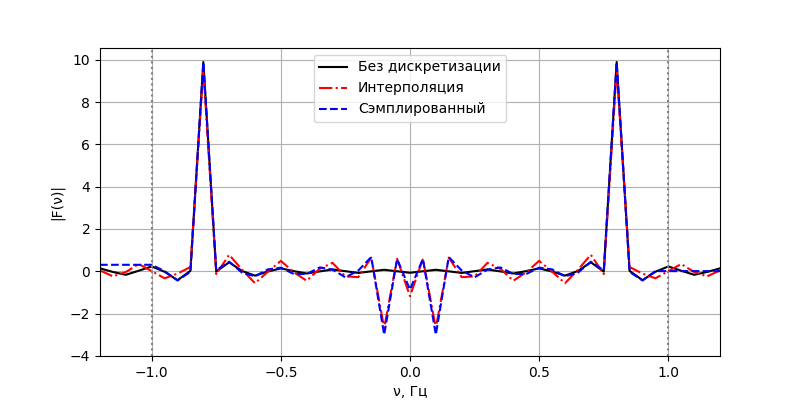
\includegraphics[width=\textwidth]{src/task_2/1_freq_10_0.5.png}
  \caption{Сравнительный график образов при $\Delta t=0.5$, $T=10$.} 
\end{figure}
\begin{figure}[H]
  \centering
  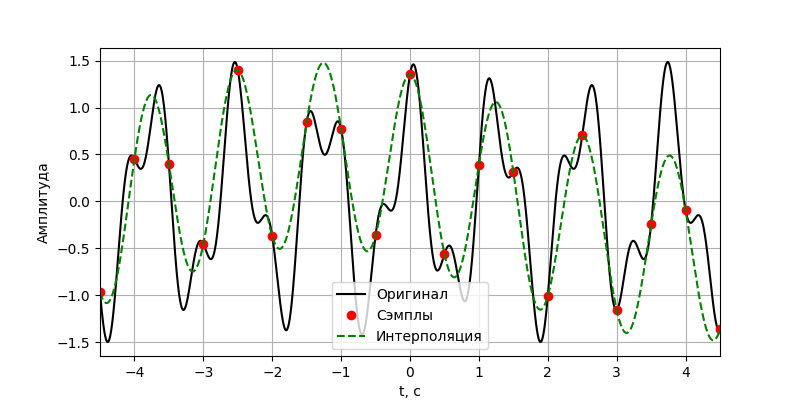
\includegraphics[width=\textwidth]{src/task_2/1_time_10_0.5.png}
  \caption{Сравнительный график при $\Delta t=0.5$, $T=10$.} 
\end{figure}
\noindent Как мы видим у метода не совсем получилось восстановить сигнал. Попробуем увеличить интервал времени \(T\) до 20 секунд и посмотрим на результаты.

\begin{figure}[H]
  \centering
  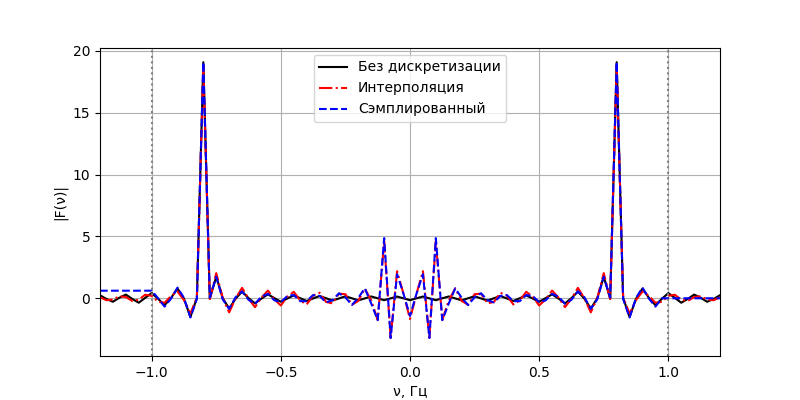
\includegraphics[width=\textwidth]{src/task_2/1_freq_20_0.5.png}
  \caption{Сравнительный график образов при $\Delta t=0.5$, $T=20$.} 
\end{figure}
\begin{figure}[H]
  \centering
  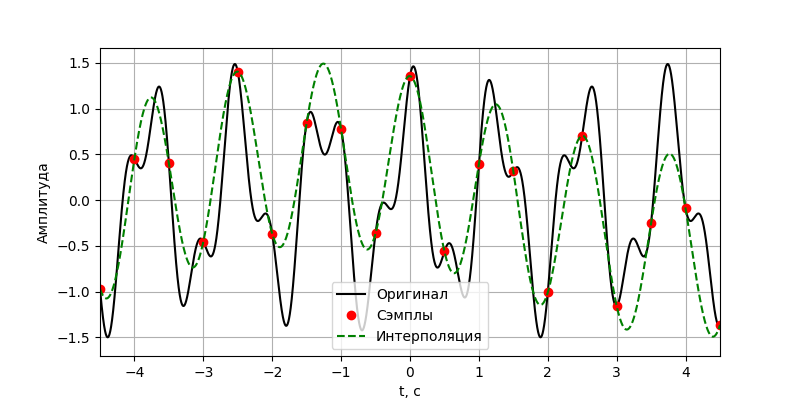
\includegraphics[width=\textwidth]{src/task_2/1_time_20_0.5.png}
  \caption{Сравнительный график при $\Delta t=0.5$, $T=20$.} 
\end{figure}

\noindent Увеличение длительности окна $T$ уменьшает шаг по частоте $\Delta\nu$, что делает спектры более «острыми», но не приходит к исходному сигналу.
Попробуем уменьшить шаг сэмплирования до \(\Delta t = 0.1\) и посмотрим на результаты.

\begin{figure}[H]
  \centering
  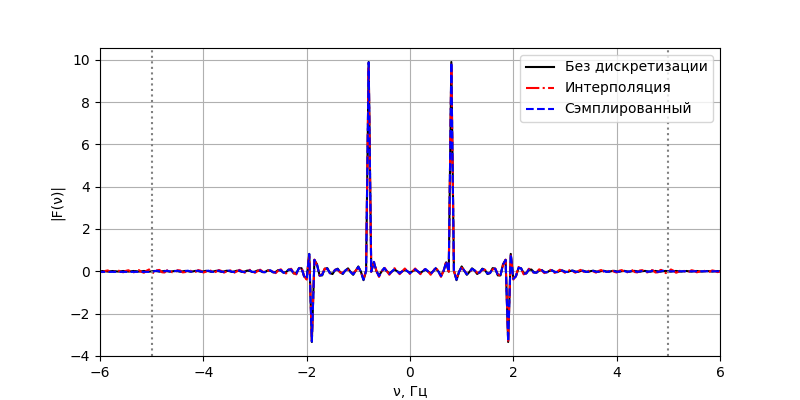
\includegraphics[width=\textwidth]{src/task_2/1_freq_10_0.1.png}
  \caption{Сравнительный график образов при $\Delta t=0.1$, $T=10$.} 
\end{figure}
\begin{figure}[H]
  \centering
  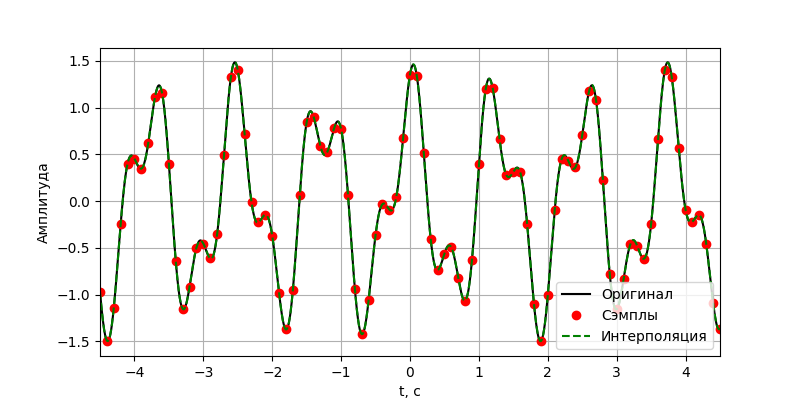
\includegraphics[width=\textwidth]{src/task_2/1_time_10_0.1.png}
  \caption{Сравнительный график при $\Delta t=0.1$, $T=10$.} 
\end{figure}
\noindent Можем заметить, что сигналы практически совпадают. Но что если увеличить интервал времени \(T\) до 20 секунд и посмотреть на результаты. 

\begin{figure}[H]
  \centering
  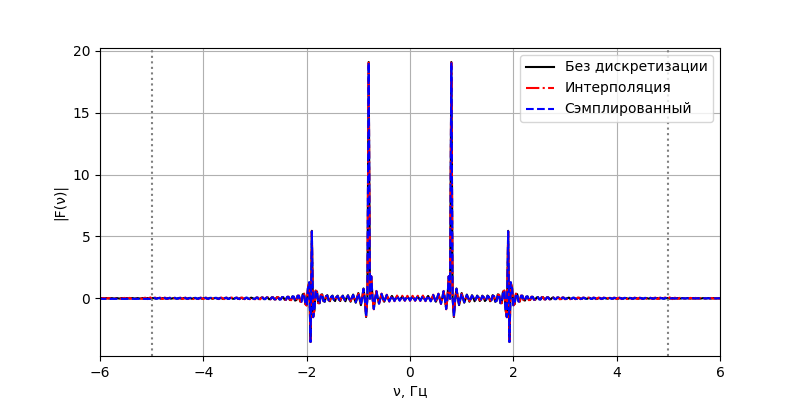
\includegraphics[width=\textwidth]{src/task_2/1_freq_20_0.1.png}
  \caption{Сравнительный график образов при $\Delta t=0.1$, $T=20$.} 
\end{figure}
\begin{figure}[H]
  \centering
  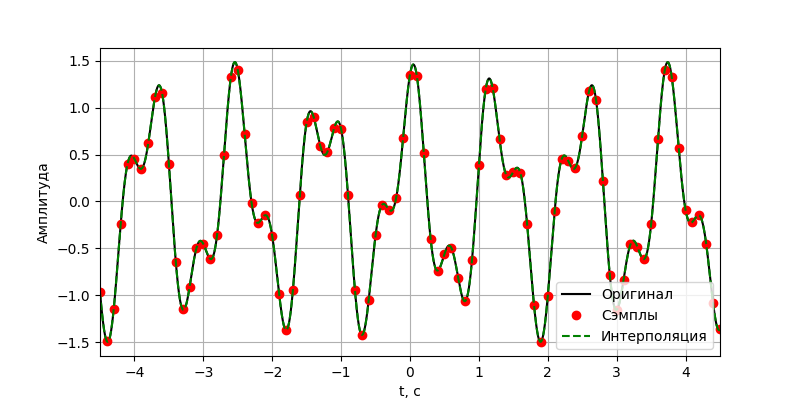
\includegraphics[width=\textwidth]{src/task_2/1_time_20_0.1.png}
  \caption{Сравнительный график при $\Delta t=0.1$, $T=20$.} 
\end{figure}
\noindent Увеличение промежутка улучшает чёткость и «остроту» спектральных пиков, при этом зона надёжного совпадения остаётся неизменной. Временная интерполяция всегда проходит через исходные точки выборки и остаётся близкой к оригиналу между ними.

Теперь попробуем восстановить вторую функцию. Для этого возьмём те же параметры и посмотрим на результаты.

\begin{figure}[H]
  \centering
  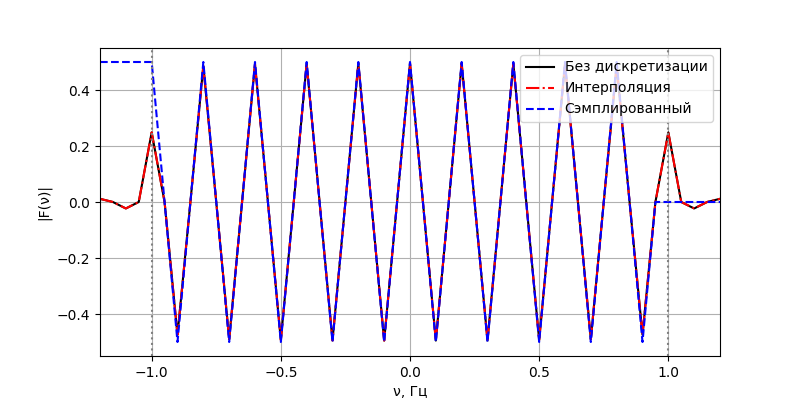
\includegraphics[width=\textwidth]{src/task_2/2_freq_10_0.5.png}
  \caption{Сравнительный график образов при $\Delta t=0.5$, $T=10$.} 
\end{figure}
\begin{figure}[H]
  \centering
  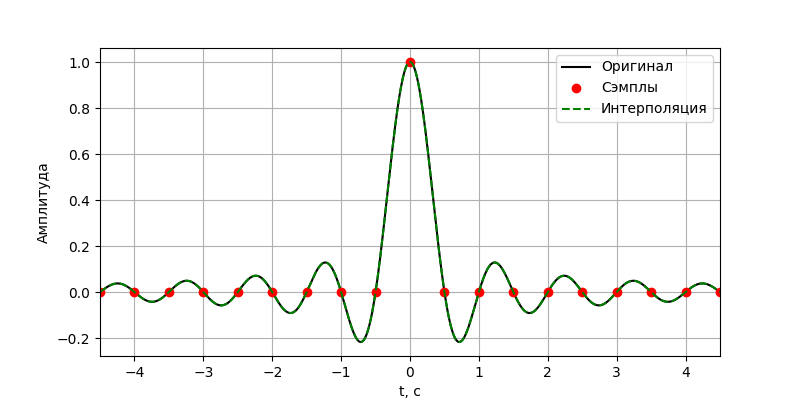
\includegraphics[width=\textwidth]{src/task_2/2_time_10_0.5.png}
  \caption{Сравнительный график при $\Delta t=0.5$, $T=10$.} 
\end{figure}

\begin{figure}[H]
  \centering
  \includegraphics[width=\textwidth]{src/task_2/2_freq_20_0.5.png}
  \caption{Сравнительный график образов при $\Delta t=0.5$, $T=20$.} 
\end{figure}
\begin{figure}[H]
  \centering
  \includegraphics[width=\textwidth]{src/task_2/2_time_20_0.5.png}
  \caption{Сравнительный график при $\Delta t=0.5$, $T=20$.} 
\end{figure}

\begin{figure}[H]
  \centering
  \includegraphics[width=\textwidth]{src/task_2/2_freq_10_0.1.png}
  \caption{Сравнительный график образов при $\Delta t=0.1$, $T=10$.} 
\end{figure}
\begin{figure}[H]
  \centering
  \includegraphics[width=\textwidth]{src/task_2/2_time_10_0.1.png}
  \caption{Сравнительный график при $\Delta t=0.1$, $T=10$.} 
\end{figure}

\begin{figure}[H]
  \centering
  \includegraphics[width=\textwidth]{src/task_2/2_freq_20_0.1.png}
  \caption{Сравнительный график образов при $\Delta t=0.1$, $T=20$.} 
\end{figure}
\begin{figure}[H]
  \centering
  \includegraphics[width=\textwidth]{src/task_2/2_time_20_0.1.png}
  \caption{Сравнительный график при $\Delta t=0.1$, $T=20$.} 
\end{figure}

Эксперимент также демонстрирует, что восстановление сигнала из сэмплов с использованием интерполяционной формулы работает корректно, если выполнены условия Найквиста, то есть частота сэмплирования достаточно высока. В случаях, когда сэмплирование происходит с недостаточной частотой, возникают эффекты алиасинга, и восстановленный сигнал существенно отличается от исходного.

\addsection{Выводы}
В ходе выполнения работы были последовательно решены две взаимосвязанные задачи:  
построение и анализ непрерывного Фурье‑преобразования прямоугольного импульса, а также изучение теоремы Найквиста–Шеннона–Котельникова.
\begin{itemize}
  \item Непрерывное FT и численные методы.  
    Метод трапеций дал высокую точность, но при этом оказался значительно медленнее.  
    Простое применение FFT было очень быстрым, однако на выходе наблюдались сдвиги и амплитудные искажения из‑за дискретизации и конечного окна.  
    Реализация «умного FFT» с фазовым множителем \(c_m\) позволила получить одновременно точный и быстрый алгоритм — совпадение с аналитическим спектром в пределах заданных параметров было практически идеальным, а обратное преобразование вернуло прямоугольный импульс без заметных артефактов.

  \item Сэмплирование и интерполяция.  
    На примере \(y_1(t)=a_1\sin(\omega_1t)+a_2\sin(\omega_2t)\) показано, что при нарушении условия \(\Delta t>1/(2B)\) высокие компоненты «сворачиваются», и никакая интерполяция не восстановит их корректно.  
    Функция \( \operatorname{sinc}(bt)\) продемонстрировала, что при строгом соблюдении \(\Delta t\le1/(2B)\) полосу сигнала можно восстановить полностью, даже если сэмплов очень мало.  
    Удлинение окна обработки \(T\) улучшает частотное разрешение, но не влияет на базовое условие безошибочной интерполяции.
\end{itemize}
\pagebreak
\addsection{Приложение}
\begin{lstlisting}[caption={Исходный код}]
import numpy as np
import matplotlib.pyplot as plt
import time

def plot_time(t, f_original, f_secondary=None, labels=['Исходная', 'Восстановленная'], xlim=None, path=None):
  plt.figure(figsize=(8,4))
  plt.plot(t, f_original, 'b-', label=labels[0])
  if f_secondary is not None:
    plt.plot(t, f_secondary, 'r--', label=labels[1])
  plt.xlabel('Время t')
  plt.ylabel('Амплитуда')
  if xlim:
    plt.xlim(xlim)
  plt.legend()
  plt.grid(True)
  if path:
    plt.savefig(path)
  plt.show()

def plot_freq(nu, F1, F2=None, labels=['Численный', 'Аналитический'], xlim=None, path=None):
  plt.figure(figsize=(8,4))
  plt.plot(nu, F1, 'b-', label=labels[0])
  if F2 is not None:
    plt.plot(nu, F2, 'r--', label=labels[1])
  plt.xlabel('Частота v')
  plt.ylabel('F(v)')
  if xlim:
    plt.xlim(xlim)
  plt.legend()
  plt.grid(True)
  if path:
    plt.savefig(path)
  plt.show()

def rect(t):
  return np.where(np.abs(t) <= 0.5, 1.0, 0.0)

def analytical_ft(nu):
  return np.sinc(nu)

def numerical_ft_trapezoid(f_t, t, nu):
  F_num = np.zeros_like(nu, dtype=complex)
  for i, freq in enumerate(nu):
    integrand = f_t * np.exp(-2j * np.pi * freq * t)
    F_num[i] = np.trapezoid(integrand, x=t)
  return F_num

def numerical_ft_extend(F_num, V, nu_extended):
  F_num_extended = np.zeros_like(nu_extended, dtype=complex)
  mask = (nu_extended >= -V) & (nu_extended < V)
  F_num_extended[mask] = F_num
  return F_num_extended

def inverse_ft_trapz(F_nu, nu, t):
  f_rec = np.zeros_like(t, dtype=complex)
  for i, time in enumerate(t):
    integrand = F_nu * np.exp(2j * np.pi * nu * time)
    f_rec[i] = np.trapezoid(integrand, x=nu)
  return f_rec

def task_1_0():
  T = 20.0
  dt = 0.01
  t = np.arange(-T/2, T/2, dt)
  V = 50
  dnu = 1 / T
  nu = np.arange(-V, V, dnu)

  f = rect(t)
  F_analytic = np.sinc(nu)

  plot_freq(nu, F_analytic, labels=['Фурье-образ'], xlim=(-7, 7))
  plot_time(t, f, labels=['П(t)'], xlim=(-1.5, 1.5))

def task_1_1():
  T_candidates = [5, 50]
  dt_candidates = [1e-2, 5e-4]
  V_candidates = [5, 20]
  dnu_candidates = [0.02, 0.5]
  ft_times = []

  for T in T_candidates:
    for dt in dt_candidates:
      t = np.arange(-T/2, T/2, dt)
      f_t = rect(t)
      for V in V_candidates:
        for dnu in dnu_candidates:
          nu = np.arange(-V, V, dnu) + dnu/2

          start_time = time.time()
          F_num = numerical_ft_trapezoid(f_t, t, nu)
          ft_time = time.time() - start_time
          ft_times.append(f"T={T}, dt={dt}, V={V}, dv={dnu}, FT time = {ft_time:.6f} s")
          f_rec = inverse_ft_trapz(F_num, nu, t).real

          print(f"T={T}, dt={dt}, V={V}, dv={dnu}, FT time = {ft_time:.6f} s")

          nu_analytic = np.arange(-V-5, V+5, dnu) + dnu/2
          F_analytic = analytical_ft(nu_analytic)
          F_num = numerical_ft_extend(F_num, V, nu_analytic)

          plot_freq(nu_analytic, F_analytic, F_num, labels=['Аналитический', 'Численный (trapezoid)'], xlim=(-V-5, V+5))
          plot_time(t, f_t, f_rec, labels=['П(t)', 'Восстановленная П(t)'], xlim=(-1.5, 1.5))
  print(*ft_times, sep='\n')

def task_1_2():
  V_fixed = 20
  dnu_fixed = 0.02

  T_candidates = [5, 10]
  dt_candidates = [2e-2, 5e-4]
  ft_times = []

  for T in T_candidates:
    for dt in dt_candidates:
      t = np.arange(-T/2, T/2, dt)
      f_t = rect(t)
      N = len(t)

      dnu = 1.0 / (N * dt)
      n = np.arange(-N//2, N//2)
      nu = n * dnu

      start_time = time.time()
      F_num = np.fft.fftshift(np.fft.fft(f_t)) * dt
      ft_time = time.time() - start_time
      ft_times.append(f"T={T}, dt={dt}, V={V_fixed}, dv={dnu}, FT time = {ft_time:.6f} s")
      f_rec = np.fft.ifft(np.fft.ifftshift(F_num)).real / dt

      print(f"T={T}, dt={dt}, V={V_fixed}, dv={dnu}, FT time = {ft_time:.6f} s")

      F_analytic = analytical_ft(nu)

      plot_freq(nu, F_analytic, F_num, labels=['Аналитический FT', 'FFT'], xlim=(-V_fixed-5, V_fixed+5))
      plot_time(t, f_t, f_rec, labels=['П(t)', 'Восстановленная П(t)'], xlim=(-1.5, 1.5))
  print(*ft_times, sep='\n')

def task_1_4():
  T_candidates = [5, 10]
  dt_candidates = [0.01, 0.0005]
  V_fixed = 20
  ft_times = []

  for T in T_candidates:
    for dt in dt_candidates:
      t = np.arange(-T/2, T/2, dt)
      f_t = rect(t)
      N = len(t)

      dnu = 1.0 / (N * dt)
      n = np.arange(-N//2, N//2)
      nu = n * dnu

      start_time = time.time()
      F_fft = np.fft.fftshift(np.fft.fft(f_t))
      ft_time = time.time() - start_time
      ft_times.append(f"T={T}, dt={dt}, V={V_fixed}, dv={dnu:.4f}, FT time = {ft_time:.6f} s")

      c = dt * np.exp(2 * np.pi * 1j * nu * (T/2))
      F_corr = F_fft * c

      F_analytic = analytical_ft(nu)

      f_rec = np.fft.ifft(np.fft.ifftshift(F_fft))

      print(f"T={T}, dt={dt}, V={V_fixed}, dv={dnu:.4f}, FT time = {ft_time:.6f} s")
      plot_freq(nu, F_analytic, F_corr, labels=['Аналитический FT', 'Умное FFT'], xlim=(-V_fixed, V_fixed))
      plot_time(t, f_t, f_rec, labels=['П(t)', 'Восстановленная П(t)'], xlim=(-1.5, 1.5))

  print(*ft_times, sep='\n')

def task_comparative():
  T = 10
  dt = 0.01
  V_fixed = 20

  t = np.arange(-T/2, T/2, dt)
  f_t = rect(t)
  N = len(t)
  ft_times = []

  dnu = 1.0 / (N * dt)
  n = np.arange(-N//2, N//2)
  nu_num = n * dnu

  nu_c = np.arange(-V_fixed, V_fixed, 0.02)
  start_time = time.time()
  F_trapz = numerical_ft_trapezoid(f_t, t, nu_c)
  ft_time = time.time() - start_time
  ft_times.append(f"Trapz: T={T}, dt={dt}, V={V_fixed}, dv={0.02}, FT time = {ft_time:.6f} s")

  f_trapz_rec = inverse_ft_trapz(F_trapz, nu_c, t).real

  start = time.time()
  F_fft = np.fft.fftshift(np.fft.fft(f_t)) * dt
  ft_time = time.time() - start
  ft_times.append(f"fft: T={T}, dt={dt}, V={V_fixed}, dv={dnu}, FT time = {ft_time:.6f} s")

  f_fft_rec = np.fft.ifft(np.fft.ifftshift(F_fft)).real / dt


  c = dt * np.exp(2 * np.pi * 1j * nu_num * (T/2))
  start = time.time()
  F_corr_fft = np.fft.fftshift(np.fft.fft(f_t))
  ft_time = time.time() - start
  ft_times.append(f"smart fft: T={T}, dt={dt}, V={V_fixed}, dv={dnu}, FT time = {ft_time:.6f} s")

  F_corr = F_corr_fft * c
  f_corr_rec = np.fft.ifft(np.fft.ifftshift(F_corr_fft))

  F_analytic = analytical_ft(nu_num)

  plt.figure(figsize=(10,6))
  plt.plot(nu_num, F_analytic, 'k--', label='Аналитический FT')
  plt.plot(nu_c, F_trapz, 'r--', label='Trapz')
  plt.plot(nu_num, F_fft, 'b--', label='Стандартный FFT', alpha=0.5)
  plt.plot(nu_num, F_corr, 'g--', label='FFT с c_m')
  plt.xlabel('Частота v')
  plt.ylabel('|F(v)|')
  plt.legend()
  plt.grid(True)
  plt.xlim(-V_fixed, V_fixed)
  plt.savefig(f"src/task_1_4/comp_freq.png")
  plt.show()

  plt.figure(figsize=(10,6))
  plt.plot(t, f_t, 'k--', label='П(t)')
  plt.plot(t, f_trapz_rec, 'r--', label='Trapz')
  plt.plot(t, f_fft_rec, 'b--', label='Стандартный FFT', alpha=0.5)
  plt.plot(t, f_corr_rec, 'g--', label='FFT с c_m')
  plt.xlabel('Время t')
  plt.ylabel('Амплитуда')
  plt.legend()
  plt.grid(True)
  plt.xlim(-1.5, 1.5)
  plt.savefig(f"src/task_1_4/comp_time.png")
  plt.show()

  print(*ft_times, sep='\n')

def y1(t, a1=1.0, a2=0.5, w1=5.0, w2=12.0, phi1=np.pi/2, phi2=np.pi/4):
  return a1*np.sin(w1*t + phi1) + a2*np.sin(w2*t + phi2)

def y2(t, b=2.0):
  return np.sinc(b * t)

def fft_smart(f_t, dt, T):
  N = len(f_t)
  dnu = 1.0 / (N * dt)
  n = np.arange(-N//2, N//2)
  nu = n * dnu
  F = np.fft.fftshift(np.fft.fft(f_t))
  c = dt * np.exp(2 * np.pi * 1j * nu * (T/2))
  F *= c
  return F, nu

def nyquist_interpolation(t_dense, t_sample, y_sample, B):
  d = t_dense[:, None] - t_sample[None, :]
  S = np.sinc(2 * B * d)
  return S.dot(y_sample)

def plot_time_signals(t_cont, y_cont, t_samp, y_samp, y_rec, path=None):
  plt.figure(figsize=(8,4))
  plt.plot(t_cont, y_cont, 'k-', label='Оригинал')
  plt.plot(t_samp, y_samp, 'ro', label='Сэмплы')
  plt.plot(t_cont, y_rec, 'g--', label='Интерполяция')
  plt.xlim(t_cont.min(), t_cont.max())
  plt.xlabel('t, с')
  plt.ylabel('Амплитуда')
  plt.xlim(-4.5, 4.5)
  plt.legend()
  plt.grid(True)
  if path:
    plt.savefig(path)
  plt.show()

def plot_spectra(nu, F_cont, F_rec, F_samp, B, path=None):
  plt.figure(figsize=(8,4))
  plt.plot(nu, F_cont, 'k-',  label='Без дискретизации')
  plt.plot(nu, F_rec, 'r-.', label='Интерполяция')
  plt.plot(nu, F_samp, 'b--', label='Сэмплированный')
  plt.axvline(B, color='gray', linestyle=':')
  plt.axvline(-B, color='gray', linestyle=':')
  plt.xlim(-1.2*B, 1.2*B)
  plt.xlabel('v, Гц')
  plt.ylabel('|F(v)|')
  plt.legend()
  plt.grid(True)
  if path:
    plt.savefig(path)
  plt.show()

def task2():
  T_list = [10, 20]
  dt_dense = 0.001
  dt_samp_list  = [0.5, 0.1]
  funcs = [y1, y2]
  for i, func in enumerate(funcs, 1):
    for T in T_list:
      t_cont = np.arange(-T, T, dt_dense)
      y_cont = func(t_cont)
      F_cont, nu = fft_smart(y_cont, dt_dense, T)

      for dt_sample in dt_samp_list:
        t_samp = np.arange(-T, T, dt_sample)
        y_samp = func(t_samp)

        B = 1 / (2 * dt_sample)

          F_samp_small, nu_samp = fft_smart(y_samp, dt_sample, T)
          F_samp = np.interp(nu, nu_samp, F_samp_small.real) \
                + 1j*np.interp(nu, nu_samp, F_samp_small.imag)

          y_rec = nyquist_interpolation(t_cont, t_samp, y_samp, B)
          F_rec, _ = fft_smart(y_rec, dt_dense, T)

          plot_time_signals(t_cont, y_cont, t_samp, y_samp, y_rec)
          plot_spectra(nu, F_cont, F_rec, F_samp, B)


if __name__ == '__main__':
  task_1_0()
  task_1_1()
  task_1_2()
  task_1_4()
  task_comparative()
  task2()
\end{lstlisting}
\end{document}